\documentclass[a4paper]{report}

% --- Paquetes ---------------------------------------------------------------
\usepackage[utf8]{inputenc}
\usepackage[a4paper,
            left=3cm, right=2.5cm,
            top=2.5cm, bottom=2.5cm]{geometry}
\usepackage{setspace}
\usepackage{fancyhdr}
\usepackage{graphicx}
\usepackage[hidelinks]{hyperref}
\usepackage{listings}
\usepackage{xcolor}
\usepackage{array}
\usepackage{tabularx}
\usepackage{booktabs}
\usepackage{longtable}
\usepackage{float}
\usepackage{url}
\usepackage{tocloft}
\usepackage{titlesec}
\usepackage{tikz}
\usepackage{amsmath}
\usepackage{enumitem}
\usepackage{microtype}
\usepackage{parskip}

% --- Fuente sans-serif (Arial equivalente) ----------------------------------
\usepackage[spanish,activeacute,es-tabla,es-noquoting]{babel}
\usepackage{helvet}
\renewcommand{\familydefault}{\sfdefault}

% --- Interlineado 1,5 -------------------------------------------------------
\onehalfspacing

% --- Colores ----------------------------------------------------------------
\definecolor{darkblue}{RGB}{0,51,102}
\definecolor{lightblue}{RGB}{173,207,230}
\definecolor{codegreen}{rgb}{0,0.55,0}
\definecolor{codegray}{rgb}{0.5,0.5,0.5}
\definecolor{codepurple}{rgb}{0.45,0,0.75}
\definecolor{backcolour}{rgb}{0.96,0.96,0.96}
\definecolor{codered}{rgb}{0.75,0,0}

% --- Listings (código fuente) -----------------------------------------------
\lstdefinestyle{mystyle}{
  backgroundcolor=\color{backcolour},
  commentstyle=\color{codegreen}\itshape,
  keywordstyle=\color{codepurple}\bfseries,
  numberstyle=\tiny\color{codegray},
  stringstyle=\color{codered},
  basicstyle=\ttfamily\footnotesize,
  breaklines=true,
  captionpos=b,
  keepspaces=true,
  numbers=left,
  numbersep=5pt,
  showspaces=false,
  showstringspaces=false,
  tabsize=2,
  frame=single,
  framesep=4pt
}
\lstset{style=mystyle}

\lstdefinelanguage{JavaScript}{
  keywords={break,case,catch,continue,default,delete,do,else,finally,
            for,function,if,in,instanceof,new,return,switch,this,throw,
            try,typeof,var,void,while,with,let,const,async,await,
            import,export,from,class,extends,super},
  keywordstyle=\color{codepurple}\bfseries,
  ndkeywords={true,false,null,undefined},
  ndkeywordstyle=\color{codered},
  sensitive=true,
  comment=[l]{//}, morecomment=[s]{/*}{*/},
  commentstyle=\color{codegreen}\itshape,
  stringstyle=\color{codered},
  morestring=[b]", morestring=[b]', morestring=[b]`
}

\lstdefinelanguage{Prisma}{
  keywords={model,datasource,generator,enum,type},
  keywordstyle=\color{codepurple}\bfseries,
  ndkeywords={String,Int,Boolean,DateTime,Float,@id,@unique,@default,
              @relation,@@unique,@@index,now,autoincrement,uuid},
  ndkeywordstyle=\color{codered},
  sensitive=true,
  comment=[l]{//},
  commentstyle=\color{codegreen}\itshape,
  stringstyle=\color{codered},
  morestring=[b]"
}

% --- Formato de títulos ------------------------------------------------------
\titleformat{\chapter}[display]
  {\normalfont\LARGE\bfseries\color{darkblue}}
  {\chaptertitlename\ \thechapter}{16pt}{\Huge}
\titlespacing*{\chapter}{0pt}{20pt}{30pt}

\titleformat{\section}
  {\normalfont\Large\bfseries\color{darkblue}}{\thesection}{1em}{}
\titlespacing*{\section}{0pt}{16pt}{8pt}

\titleformat{\subsection}
  {\normalfont\large\bfseries\color{darkblue}}{\thesubsection}{1em}{}
\titlespacing*{\subsection}{0pt}{12pt}{6pt}

\titleformat{\subsubsection}
  {\normalfont\normalsize\bfseries\color{darkblue}}{\thesubsubsection}{1em}{}

% --- Cabeceras y pies --------------------------------------------------------
\pagestyle{fancy}
\fancyhf{}
\fancyhead[L]{\small\leftmark}
\fancyhead[R]{\small FPConnect -- TFG DAM}
\fancyfoot[C]{\thepage}
\renewcommand{\headrulewidth}{0.4pt}
\setlength{\headheight}{14pt}

% --- Hipervínculos -----------------------------------------------------------
\hypersetup{
  colorlinks=true,
  linkcolor=darkblue,
  citecolor=darkblue,
  urlcolor=darkblue
}

% ════════════════════════════════════════════════════════════════════════════
\begin{document}
% ════════════════════════════════════════════════════════════════════════════

% --- PORTADA ----------------------------------------------------------------
\begin{titlepage}
  \thispagestyle{empty}
  \centering

  % Logo del centro
  \vspace*{0.5cm}
  
\includegraphics[width=5cm]{images/logo.png}

  \vspace*{1.5cm}

  {\fontsize{36}{42}\selectfont\bfseries\color{darkblue} FPCONNECT \par}

  \vspace{0.6cm}
  {\fontsize{20}{24}\selectfont\bfseries Red Social de Formación Profesional \par}

  \vspace{1cm}
  \textcolor{darkblue}{\rule{12cm}{1pt}}
  \vspace{0.8cm}

  {\fontsize{13}{16}\selectfont\itshape
  Plataforma web y de escritorio para conectar alumnos de FP,\\[4pt]
  centros educativos y empresas en Andalucía \par}

  \vfill

  {\fontsize{12}{15}\selectfont
  \begin{tabular}{rl}
    \textbf{Tipo de trabajo:} & Trabajo Final de Grado \\[6pt]
    \textbf{Ciclo:}           & Desarrollo de Aplicaciones Multiplataforma (DAM) \\[6pt]
    \textbf{Centro:}          & CES Lope de Vega \\[6pt]
    \textbf{Curso:}           & 2025/2026 \\[6pt]
    \textbf{Fecha de entrega:}& \today \\
  \end{tabular}
  \par}

  \vspace{2cm}
  \textcolor{darkblue}{\rule{12cm}{1pt}}
\end{titlepage}

% --- ÍNDICE -----------------------------------------------------------------
\pagestyle{fancy}
\tableofcontents
\newpage

% ════════════════════════════════════════════════════════════════════════════
\chapter*{Resumen}
\addcontentsline{toc}{chapter}{Resumen}
% ════════════════════════════════════════════════════════════════════════════

FPConnect es una plataforma web y de escritorio innovadora diseñada específicamente para el sector de la Formación Profesional en Andalucía. El objetivo principal es crear un ecosistema digital que conecte a estudiantes de FP, centros educativos y empresas del sector productivo, facilitando la búsqueda de oportunidades laborales, el intercambio de conocimiento y la construcción de redes profesionales significativas.

La plataforma integra funcionalidades de red social profesional con herramientas especializadas para el sector de FP, permitiendo que los usuarios compartan experiencias, busquen ofertas de empleo, se conecten con empresas y accedan a recursos educativos. A diferencia de plataformas genéricas como LinkedIn, FPConnect está concebida exclusivamente para el ecosistema de la Formación Profesional andaluza, con un diseño de roles que diferencia entre alumnos, centros y empresas, cada uno con sus propias vistas, funcionalidades y necesidades.

Desde el punto de vista técnico, FPConnect ha sido desarrollado utilizando tecnologías modernas y escalables: React~18 con Vite en el frontend, Node.js/Express en el backend, PostgreSQL como gestor de base de datos y Socket.io para la comunicación en tiempo real. Esta arquitectura garantiza un sistema robusto, seguro y capaz de crecer con las demandas futuras.

El proyecto ha sido desarrollado siguiendo una metodología Agile con sprints regulares, iteraciones continuas y validación con usuarios reales del sector educativo. Se ha implementado un sistema de autenticación robusto con soporte para OAuth con Google, validaciones exhaustivas en cliente y servidor, y medidas de seguridad avanzadas para proteger los datos de los usuarios.

Esta documentación detalla todas las fases del desarrollo del proyecto, desde la conceptualización inicial hasta la validación final, describiendo cómo se han alcanzado los objetivos propuestos y señalando las vías de mejora para futuras iteraciones.

\bigskip
\noindent\textbf{Palabras clave:} red social, Formación Profesional, Andalucía, React, Node.js, PostgreSQL, Socket.io, JWT, Prisma, REST API, tiempo real, multiplataforma.

\bigskip
\noindent\textbf{Keywords:} social network, Vocational Training, Andalusia, React, Node.js, PostgreSQL, Socket.io, JWT, Prisma, REST API, real-time, multiplatform.

\newpage

% ════════════════════════════════════════════════════════════════════════════
\chapter*{Glosario}
\addcontentsline{toc}{chapter}{Glosario}
% ════════════════════════════════════════════════════════════════════════════

\begin{description}[leftmargin=3.5cm, style=nextline]

  \item[\textbf{API}] \textit{(Application Programming Interface)} Interfaz de programación que permite la comunicación entre diferentes aplicaciones y servicios de forma estandarizada y automatizada.

  \item[\textbf{Backend}] Parte servidora de una aplicación donde se procesa la lógica de negocio, las validaciones y el acceso a bases de datos. No es visible directamente por el usuario.

  \item[\textbf{Bcrypt}] Algoritmo de \textit{hashing} criptográfico especializado en el almacenamiento seguro de contraseñas, con factor de coste configurable para adaptarse a la potencia del hardware disponible.

  \item[\textbf{CORS}] \textit{(Cross-Origin Resource Sharing)} Mecanismo de seguridad del navegador que controla qué orígenes externos pueden acceder a los recursos de un servidor.

  \item[\textbf{Docker}] Plataforma de contenerización que permite empaquetar aplicaciones junto con todas sus dependencias, garantizando un comportamiento idéntico en cualquier entorno.

  \item[\textbf{Escalabilidad}] Capacidad de un sistema para gestionar un aumento progresivo en la carga de usuarios y datos sin degradar significativamente su rendimiento.

  \item[\textbf{FCT}] \textit{(Formación en Centro de Trabajo)} Período de prácticas en empresa que forma parte del currículo oficial de los ciclos formativos de Formación Profesional en España.

  \item[\textbf{Frontend}] Interfaz visual de una aplicación web o móvil con la que interactúa directamente el usuario final.

  \item[\textbf{HMR}] \textit{(Hot Module Replacement)} Técnica de desarrollo que actualiza módulos de una aplicación en el navegador en tiempo real sin necesidad de recargar la página completa.

  \item[\textbf{JWT}] \textit{(JSON Web Token)} Estándar abierto (RFC 7519) para autenticación \textit{stateless} que permite transmitir información firmada digitalmente entre cliente y servidor.

  \item[\textbf{Leaflet}] Librería JavaScript de código abierto para crear mapas interactivos en aplicaciones web, con soporte para marcadores, capas y eventos geoespaciales.

  \item[\textbf{Middleware}] Software intermediario que procesa las solicitudes HTTP antes de que lleguen al controlador final, permitiendo tareas como validación, autenticación o registro.

  \item[\textbf{OAuth}] Protocolo de autorización estándar que permite a los usuarios autenticarse en una aplicación utilizando credenciales de un proveedor externo (p.~ej. Google).

  \item[\textbf{ORM}] \textit{(Object-Relational Mapping)} Herramienta que traduce automáticamente objetos de programación a filas de tablas de una base de datos relacional y viceversa.

  \item[\textbf{PostgreSQL}] Sistema de gestión de base de datos relacional de código abierto, con soporte para transacciones ACID, JSON nativo y alta extensibilidad.

  \item[\textbf{Prisma}] ORM moderno para Node.js que proporciona \textit{type-safety}, generación automática de migraciones y un cliente de base de datos con autocompletado.

  \item[\textbf{Rate Limiting}] Técnica para limitar el número de solicitudes que un cliente puede realizar a un servidor en un intervalo de tiempo, protegiéndolo contra ataques de fuerza bruta o abuso.

  \item[\textbf{React}] Librería JavaScript desarrollada por Meta para construir interfaces de usuario reactivas basadas en componentes reutilizables.

  \item[\textbf{REST}] \textit{(Representational State Transfer)} Estilo arquitectónico para servicios web que utiliza los métodos HTTP estándar (GET, POST, PUT, DELETE) y recursos identificados por URL.

  \item[\textbf{Socket.io}] Librería que implementa comunicación bidireccional y en tiempo real entre cliente y servidor mediante WebSockets, con \textit{fallback} automático a otros transportes.

  \item[\textbf{SPA}] \textit{(Single Page Application)} Aplicación web que carga una única página HTML y actualiza dinámicamente su contenido mediante JavaScript, sin recargas completas del navegador.

  \item[\textbf{Tailwind CSS}] \textit{Framework} de CSS basado en clases utilitarias que permite diseñar interfaces directamente en el marcado HTML sin abandonar el fichero de componente.

  \item[\textbf{Tauri}] \textit{Framework} para crear aplicaciones de escritorio multiplataforma usando tecnologías web (HTML, CSS, JavaScript) con un binario nativo muy ligero basado en Rust.

  \item[\textbf{Vite}] Herramienta moderna de construcción y empaquetado para el frontend que ofrece HMR ultrarrápido y una configuración mínima lista para producción.

  \item[\textbf{WebSocket}] Protocolo de comunicación bidireccional y persistente entre cliente y servidor sobre una única conexión TCP, ideal para aplicaciones en tiempo real.

  \item[\textbf{Zustand}] Librería de gestión de estado global para React, ligera y sin \textit{boilerplate}, basada en un modelo de tienda inmutable y selectores reactivos.

\end{description}

\newpage

% ════════════════════════════════════════════════════════════════════════════
\chapter{Planteamiento del Problema y Justificación}
% ════════════════════════════════════════════════════════════════════════════

\section{Contexto del sector}

La Formación Profesional en Andalucía constituye uno de los pilares fundamentales del sistema educativo regional. Según datos de la Junta de Andalucía, más de 250.000 estudiantes están matriculados en ciclos formativos de grado medio y superior, con una tendencia de crecimiento sostenido en los últimos años. Sin embargo, pese a este volumen, el ecosistema digital que conecta a estos actores (alumnos, centros y empresas) sigue siendo fragmentado e ineficiente.

Las empresas del sector productivo andaluz manifiestan dificultades para localizar perfiles técnicos específicos procedentes de la FP, mientras que los propios estudiantes reconocen no disponer de canales adecuados para visibilizar sus competencias o encontrar oportunidades formativas y laborales ajustadas a su especialidad. Los centros educativos, por su parte, carecen de herramientas digitales propias que les permitan actuar como puente entre ambos colectivos.

\section{Necesidades identificadas}

A partir del análisis del sector y de conversaciones con usuarios reales (alumnos, docentes y responsables de selección de personal), se identificaron las siguientes necesidades no cubiertas:

\subsection{Ausencia de plataforma especializada}

No existe ninguna red social ni plataforma digital diseñada específicamente para el ecosistema de la FP española o andaluza. Las soluciones existentes son generalistas y no contemplan la estructura de roles, ciclos formativos, módulos profesionales ni la FCT. Los estudiantes se ven obligados a utilizar LinkedIn, una herramienta pensada para perfiles universitarios y profesionales senior, con una curva de aprendizaje y una orientación que no se adapta a sus necesidades.

\subsection{Dificultad en la búsqueda de prácticas y empleo}

La búsqueda de empresa para la FCT sigue dependiendo en muchos casos de contactos personales del profesorado o de llamadas telefónicas. No existe un canal estructurado donde las empresas publiquen sus necesidades de alumnos en prácticas y los estudiantes puedan candidatarse de forma directa y pública.

\subsection{Falta de networking sectorial}

Construir una red profesional es una de las habilidades más valoradas en el mercado laboral actual. Sin embargo, los alumnos de FP no disponen de un espacio digital donde conectar con exalumnos de su mismo ciclo, con profesionales del sector o con docentes que puedan actuar como mentores.

\subsection{Comunicación fragmentada entre actores}

La comunicación entre centros educativos, alumnos y empresas se apoya en correo electrónico, teléfono o grupos informales de mensajería instantánea. No hay un canal unificado, profesional y trazable que permita gestionar estas interacciones con eficiencia.

\section{Análisis de soluciones existentes}

Se ha llevado a cabo un análisis comparativo de las principales plataformas disponibles en el mercado para identificar los huecos que FPConnect puede cubrir.

\subsection{LinkedIn}

LinkedIn es la red social profesional más extendida a nivel mundial, con más de mil millones de usuarios registrados. Ofrece funcionalidades sólidas de networking, búsqueda de empleo y publicación de contenido profesional. Sin embargo, su diseño está orientado a perfiles universitarios y directivos, y sus filtros de búsqueda no contemplan conceptos propios de la FP como ciclo formativo, módulo profesional o familia profesional. Además, su interfaz resulta compleja para usuarios jóvenes que se incorporan por primera vez al mercado laboral.

\subsection{Portales de empleo generales (Indeed, Infojobs)}

Estos portales agregan ofertas de trabajo y permiten subir un currículum, pero carecen por completo de funcionalidades de red social, mensajería o creación de comunidad. Tampoco permiten distinguir entre ofertas de empleo ordinario y plazas específicas para alumnos en FCT.

\subsection{Redes sociales genéricas}

Plataformas como Instagram o TikTok son ampliamente utilizadas por jóvenes, pero no ofrecen ninguna funcionalidad orientada al empleo o a la construcción de una identidad profesional.

\section{Propuesta de valor de FPConnect}

FPConnect se posiciona como la primera plataforma digital diseñada específicamente para el ecosistema de la Formación Profesional andaluza. Su propuesta de valor se articula en torno a tres ejes:

\begin{enumerate}
  \item \textbf{Especialización sectorial:} roles diferenciados para alumnos, centros y empresas, con campos de perfil, filtros de búsqueda y funcionalidades adaptadas a cada uno.
  \item \textbf{Comunidad y networking:} feed social, sistema de conexiones bidireccionales y mensajería privada en tiempo real para construir relaciones profesionales significativas.
  \item \textbf{Intermediación laboral:} módulo de ofertas de empleo y FCT donde las empresas publican sus necesidades y los alumnos pueden candidatarse directamente.
\end{enumerate}

\newpage

% ════════════════════════════════════════════════════════════════════════════
\chapter{Fundamentación Teórica y Estado del Arte}
% ════════════════════════════════════════════════════════════════════════════

\section{Redes sociales profesionales: bases conceptuales}

El concepto de red social como estructura que modela las relaciones entre actores fue introducido en las ciencias sociales por Barnes (1954) y formalizado matemáticamente en la teoría de grafos. En el ámbito digital, Boyd y Ellison (2007) definieron las redes sociales en internet como servicios web que permiten a los individuos construir un perfil público o semipúblico, articular una lista de usuarios con quienes comparten alguna conexión e interactuar con dicha red. Esta definición sigue siendo la referencia fundamental en los estudios sobre plataformas digitales sociales.

Las redes sociales profesionales, como subconjunto de este fenómeno, añaden la dimensión del capital social orientado al mercado laboral. Según Granovetter (1973), los llamados \textit{lazos débiles} (conocidos lejanos, contactos de segundo grado) son con frecuencia más útiles que los lazos fuertes para encontrar empleo, ya que actúan como puentes hacia círculos de información distintos. Este principio fundamenta el diseño de plataformas como LinkedIn y, por extensión, FPConnect.

\section{Arquitecturas web modernas}

\subsection{Evolución de los frameworks frontend}

El desarrollo de aplicaciones web ha evolucionado notablemente desde los primeros modelos de renderizado en servidor. Durante la primera generación de frameworks (2000--2010), toda la lógica de presentación residía en el servidor, que generaba HTML completo en cada solicitud. Con la aparición de AJAX y herramientas como jQuery, se introdujo la posibilidad de actualizar partes de la página sin recargarla.

La segunda generación (2010--2015) trajo consigo los primeros frameworks de SPA: Angular 1.x, Backbone.js y Ember.js, que trasladaron gran parte de la lógica al cliente. La tercera generación, iniciada en 2013 con React, introdujo el concepto de Virtual DOM y el modelo de programación declarativa basada en componentes, que hoy domina el desarrollo web frontend. Según la encuesta anual de Stack Overflow de 2024, React es el framework web más utilizado por los desarrolladores a nivel mundial, con una cuota de más del 40\%.

\subsection{Arquitectura REST y APIs}

El estilo arquitectónico REST (\textit{Representational State Transfer}), definido por Roy Fielding en su tesis doctoral de 2000, establece un conjunto de restricciones para el diseño de servicios web sobre HTTP. Sus principios fundamentales (interfaz uniforme, arquitectura cliente-servidor, ausencia de estado, caché, sistema de capas y código bajo demanda) han sido ampliamente adoptados como estándar de facto para el diseño de APIs en aplicaciones web modernas.

En FPConnect, la API REST expone recursos identificados por URI (usuarios, posts, mensajes, notificaciones) y opera mediante los métodos HTTP estándar, garantizando interoperabilidad y facilidad de integración con clientes de cualquier naturaleza.

\subsection{Comunicación en tiempo real: WebSockets}

El protocolo WebSocket (RFC 6455, 2011) establece un canal de comunicación bidireccional y persistente entre cliente y servidor sobre una única conexión TCP. A diferencia del modelo HTTP de solicitud/respuesta, los WebSockets permiten al servidor enviar datos al cliente en cualquier momento sin necesidad de que este los solicite explícitamente. Esta característica es fundamental para implementar funcionalidades como la mensajería instantánea o las notificaciones en tiempo real.

Socket.io, la librería utilizada en FPConnect, abstrae la complejidad del protocolo WebSocket y añade funcionalidades como reconexión automática, \textit{fallback} a \textit{long-polling} HTTP cuando WebSocket no está disponible, y un modelo de eventos que simplifica el desarrollo.

\section{Seguridad en aplicaciones web}

\subsection{OWASP Top 10}

La Open Web Application Security Project (OWASP) publica periódicamente una lista de los diez riesgos de seguridad más críticos en aplicaciones web. La edición de 2021 incluye, entre otros, la inyección SQL, las fallas de autenticación, la exposición de datos sensibles y la configuración incorrecta de seguridad. El diseño de FPConnect ha tenido en cuenta esta guía de referencia desde las primeras etapas del proyecto.

\subsection{Autenticación basada en tokens: JWT}

JSON Web Token (JWT) es un estándar abierto (RFC 7519) que define un formato compacto y autocontenido para transmitir información entre partes como un objeto JSON firmado digitalmente. Frente a los mecanismos de sesión tradicionales basados en cookies y almacenamiento en servidor, los JWT permiten implementar autenticación \textit{stateless}, lo que facilita la escalabilidad horizontal de la aplicación ya que el servidor no necesita mantener un registro de sesiones activas.

\subsection{Almacenamiento seguro de contraseñas}

El almacenamiento de contraseñas en texto plano o con funciones de hash no adecuadas (MD5, SHA-1) es una vulnerabilidad crítica documentada en múltiples brechas de datos. Provos y Mazières (1999) propusieron el algoritmo bcrypt como solución específica para el hashing de contraseñas, con un factor de coste ajustable que permite adaptar el tiempo de cómputo al hardware disponible y dificultar los ataques de fuerza bruta.

\section{Bases de datos relacionales y ORM}

PostgreSQL es uno de los sistemas gestores de bases de datos relacionales de código abierto más avanzados disponibles. Su soporte para transacciones ACID, tipos de datos avanzados (incluido JSON nativo mediante el tipo JSONB), índices parciales y funciones almacenadas lo convierte en una opción robusta para aplicaciones de producción.

Prisma es un ORM de nueva generación para Node.js que introduce el concepto de \textit{schema-first development}: el desarrollador define el modelo de datos en un fichero \texttt{schema.prisma} y Prisma genera automáticamente el cliente de base de datos con tipado estático completo, así como las migraciones SQL necesarias para mantener la base de datos sincronizada con el modelo.

\section{Metodologías de desarrollo ágil}

El Manifiesto Ágil (Beck et al., 2001) estableció los valores y principios que sustentan las metodologías de desarrollo iterativo e incremental. Entre sus principios fundamentales destaca la entrega continua de software funcional, la adaptación a los cambios de requisitos y la colaboración estrecha con el cliente. FPConnect ha sido desarrollado siguiendo un enfoque Agile con sprints de dos semanas, revisión de resultados al final de cada iteración y ajuste del \textit{backlog} en función de la retroalimentación recibida.

\newpage

% ════════════════════════════════════════════════════════════════════════════
\chapter{Objetivos}
% ════════════════════════════════════════════════════════════════════════════

\section{Objetivo principal}

Desarrollar FPConnect, una plataforma web y de escritorio que actúe como red social profesional especializada para el sector de la Formación Profesional en Andalucía, facilitando la conexión efectiva entre alumnos, centros educativos y empresas mediante funcionalidades de perfil diferenciado, feed social, mensajería en tiempo real, sistema de conexiones y módulo de ofertas de empleo.

\section{Objetivos específicos}

\begin{enumerate}
  \item Implementar un sistema de autenticación seguro con soporte para múltiples métodos de acceso: email y contraseña, y OAuth con Google mediante Passport.js.
  \item Diseñar perfiles de usuario diferenciados por rol (alumno, centro, empresa) con campos y funcionalidades específicas para cada tipo de actor.
  \item Desarrollar un feed social donde los usuarios puedan publicar contenido profesional, comentar e interactuar mediante reacciones.
  \item Crear un sistema de conexiones bidireccionales con estados (pendiente, aceptada, rechazada) que permita construir redes profesionales reales.
  \item Implementar un módulo de mensajería privada en tiempo real mediante WebSockets (Socket.io) con persistencia de historial.
  \item Desarrollar un sistema de notificaciones en tiempo real que informe a los usuarios sobre interacciones y eventos relevantes.
  \item Crear funcionalidades de búsqueda y filtrado avanzadas para encontrar usuarios, ofertas y contenido específico por rol, especialidad o ubicación.
  \item Implementar un panel de control personalizado según el rol del usuario, con estadísticas e información relevante.
  \item Garantizar la seguridad de la plataforma mediante autenticación JWT, hashing de contraseñas con bcrypt, protección contra vulnerabilidades OWASP (XSS, inyección SQL, CSRF) y \textit{rate limiting}.
  \item Asegurar un rendimiento adecuado con tiempos de respuesta inferiores a 200~ms en operaciones de lectura habituales.
  \item Desplegar la aplicación en infraestructura en la nube con pipeline de CI/CD automatizado.
\end{enumerate}

\newpage

% ════════════════════════════════════════════════════════════════════════════
\chapter{Metodología}
% ════════════════════════════════════════════════════════════════════════════

\section{Enfoque metodológico}

El proyecto FPConnect ha sido desarrollado siguiendo una metodología ágil basada en los principios del Manifiesto Ágil, adaptada a un contexto de desarrollo individual. El ciclo de trabajo se ha organizado en sprints de dos semanas, con revisión de objetivos al final de cada iteración y actualización del \textit{backlog} en función del progreso real.

La elección de una metodología ágil frente a un enfoque en cascada (\textit{waterfall}) responde a la naturaleza cambiante de los requisitos en el desarrollo de aplicaciones web: las necesidades de los usuarios se clarifican a medida que interactúan con prototipos funcionales, y la arquitectura técnica debe poder adaptarse sin comprometer el trabajo ya realizado.

\section{Fases del proyecto}

\subsection{Fase 1: Análisis y diseño (semanas 1--2)}

Durante las dos primeras semanas se llevaron a cabo las siguientes actividades:

\begin{itemize}
  \item Análisis de necesidades del sector mediante entrevistas informales con alumnos de FP, docentes y responsables de RRHH de empresas.
  \item Análisis comparativo de plataformas existentes (LinkedIn, Indeed, Infojobs).
  \item Definición de requisitos funcionales y no funcionales.
  \item Diseño de la arquitectura del sistema (tres capas: presentación, aplicación y datos).
  \item Diseño del modelo de datos y elaboración del \textit{schema} inicial de Prisma.
  \item Creación de \textit{wireframes} para las principales vistas de la aplicación.
  \item Planificación del \textit{backlog} de sprints.
\end{itemize}

\begin{figure}[H]
  \centering
  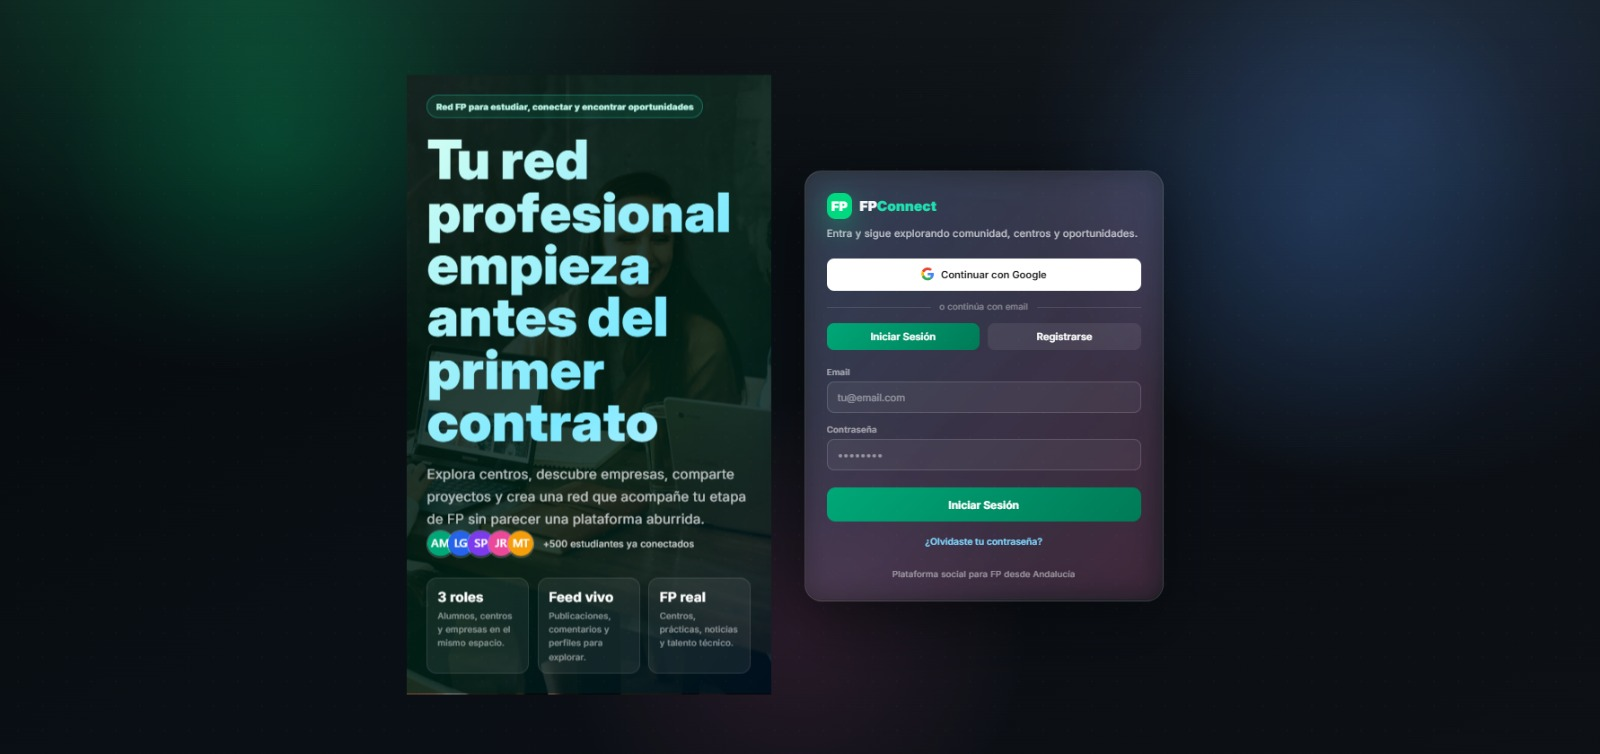
\includegraphics[width=0.7\textwidth]{images/02_signup_form.jpg}
  \caption{Prototipo de wireframe: Pantalla de registro con selección de roles (Alumno, Centro, Empresa)}
  \label{fig:wireframe_login}
\end{figure}

\subsection{Fase 2: Configuración del entorno (semana 3)}

\begin{itemize}
  \item Creación del repositorio Git con política de ramas (\textit{main}, \textit{develop}, \textit{feature/*}).
  \item Configuración de Docker Compose para levantar PostgreSQL, backend y frontend en local con un único comando.
  \item Setup inicial del proyecto frontend con Vite y React, y del proyecto backend con Node.js y Express.
  \item Configuración de ESLint, Prettier y los scripts de \textit{testing}.
  \item Configuración de las variables de entorno y fichero \texttt{.env.example}.
\end{itemize}

\subsection{Fase 3: Desarrollo del backend (semanas 4--6)}

Desarrollo de la API REST y la lógica de servidor:

\begin{itemize}
  \item Definición completa del \textit{schema} de Prisma y ejecución de migraciones.
  \item Implementación del sistema de autenticación: registro, login con JWT, integración de Passport.js para OAuth con Google (\texttt{googleAuth.routes.js}).
  \item Desarrollo de controladores y servicios para cada recurso: usuarios, posts, comentarios, conexiones, mensajes, notificaciones y ofertas de empleo.
  \item Implementación de los \textit{middlewares}: autenticación JWT (\texttt{auth.js}), manejo centralizado de errores (\texttt{errorHandler.js}) y validación de entradas (\texttt{validation.js}).
  \item Configuración de Socket.io para mensajería en tiempo real (\texttt{sockets/messaging.socket.js}).
  \item Implementación del \texttt{responseHandler.js} como utilidad para normalizar todas las respuestas de la API.
  \item Creación de \textit{seeds} para poblar la base de datos con datos de prueba (\texttt{seed.js}, \texttt{seed-alumnos.js}).
  \item Script de administración para recuperación de cuentas (\texttt{admin-set-recovery.js}).
  \item Escritura de tests: \texttt{auth.test.js}, \texttt{posts.test.js}, \texttt{offers.test.js} con \texttt{testUtils.js} y \texttt{\_\_mocks\_\_}.
\end{itemize}

\subsection{Fase 4: Desarrollo del frontend (semanas 7--9)}

\begin{itemize}
  \item Estructura de carpetas con separación entre páginas, componentes, servicios, \textit{store} y \textit{hooks}.
  \item Desarrollo de componentes de \textit{layout} (Header, Sidebar, Layout).
  \item Implementación de páginas principales: Login, Registro, Feed, Perfil, Búsqueda, Dashboard, Mensajes.
  \item Integración con la API mediante Axios con interceptores para inyección automática del token JWT.
  \item Gestión de estado global con Zustand (\texttt{authStore.js}, \texttt{postStore.js}, \texttt{notificationStore.js}).
  \item Integración de Socket.io en el cliente mediante el \textit{hook} personalizado \texttt{useSocket.js}.
  \item Estilos con Tailwind CSS.
  \item Enrutamiento protegido por rol con React Router v6.
\end{itemize}

\subsection{Fase 5: Testing y validación (semana 10)}

\begin{itemize}
  \item Ejecución de la suite de tests automatizados y corrección de errores detectados.
  \item Pruebas de carga con Artillery para validar el comportamiento bajo estrés.
  \item Pruebas de usabilidad con cinco usuarios reales del sector FP.
  \item Revisión de accesibilidad y corrección de contrastes.
\end{itemize}

\subsection{Fase 6: Documentación y despliegue (semanas 10--11)}

\begin{itemize}
  \item Redacción de la documentación técnica: \texttt{README.md}, \texttt{ARCHITECTURE.md}, \texttt{DATABASE\_SETUP.md}, \texttt{API\_ENDPOINTS.md}, \texttt{ENDPOINTS\_SUMMARY.md}, \texttt{FRONTEND\_INTEGRATION.md}.
  \item Configuración del pipeline de CI/CD con GitHub Actions.
  \item Despliegue del backend en Railway y del frontend en Vercel.
  \item Redacción de la presente memoria del TFG.
\end{itemize}

\section{Herramientas utilizadas}

\begin{table}[H]
  \centering
  \begin{tabularx}{\textwidth}{lX}
    \toprule
    \textbf{Herramienta} & \textbf{Uso en el proyecto} \\
    \midrule
    Visual Studio Code    & Editor de código principal \\
    Git / GitHub          & Control de versiones y repositorio remoto \\
    Docker / Docker Compose & Entorno de desarrollo local reproducible \\
    Postman               & Pruebas manuales de la API REST \\
    Artillery             & Pruebas de rendimiento y carga \\
    GitHub Actions        & Pipeline de integración y entrega continua \\
    Figma                 & Diseño de \textit{wireframes} y prototipos \\
    Notion                & Gestión del \textit{backlog} y planificación de sprints \\
    \bottomrule
  \end{tabularx}
  \caption{Herramientas utilizadas durante el desarrollo del proyecto}
\end{table}

\section{Distribución temporal}

\begin{table}[H]
  \centering
  \begin{tabular}{lrr}
    \toprule
    \textbf{Fase} & \textbf{Semanas} & \textbf{Horas estimadas} \\
    \midrule
    Fase 1: Análisis y diseño          & 1--2   & 80  \\
    Fase 2: Configuración del entorno  & 3      & 40  \\
    Fase 3: Desarrollo del backend     & 4--6   & 120 \\
    Fase 4: Desarrollo del frontend    & 7--9   & 120 \\
    Fase 5: Testing y validación       & 10     & 80  \\
    Fase 6: Documentación y despliegue & 10--11 & 60  \\
    \midrule
    \textbf{Total}                     &        & \textbf{500} \\
    \bottomrule
  \end{tabular}
  \caption{Distribución de horas por fase del proyecto}
\end{table}

\section{Evaluación de costes}

\subsection{Recursos humanos}

Considerando una tarifa orientativa de 25~€/hora para un desarrollador junior en Andalucía:

\[
  500\text{ horas} \times 25\text{ €/hora} = \mathbf{12.500\text{ €}}
\]

\subsection{Tecnologías}

Todas las tecnologías principales del proyecto son de código abierto y gratuitas: React (licencia MIT), Node.js/Express (licencia MIT), PostgreSQL (licencia PostgreSQL), Prisma (Apache 2.0), Docker (gratuito para uso personal/educativo). Coste total de software: \textbf{0~€}.

\subsection{Infraestructura en producción}

\begin{table}[H]
  \centering
  \begin{tabular}{lrr}
    \toprule
    \textbf{Servicio} & \textbf{Coste/mes} & \textbf{Coste/año} \\
    \midrule
    Railway (backend + BD) & 15~€ & 180~€ \\
    Vercel (frontend)      & 0--20~€ & 0--240~€ \\
    Dominio .app           & ---  & 14~€ \\
    \midrule
    \textbf{Total estimado} & \textbf{15--35~€} & \textbf{194--434~€} \\
    \bottomrule
  \end{tabular}
  \caption{Estimación de costes de infraestructura en producción}
\end{table}

\newpage

% ════════════════════════════════════════════════════════════════════════════
\chapter{Resultados}
% ════════════════════════════════════════════════════════════════════════════

\section{Arquitectura del sistema}

FPConnect implementa una arquitectura de tres capas (\textit{Three-Tier Architecture}) que separa las responsabilidades en niveles distintos, garantizando mantenibilidad, escalabilidad y separación de responsabilidades.

\begin{figure}[H]
\centering
\begin{tikzpicture}[
  layer/.style={rectangle, draw=darkblue, fill=lightblue!30,
                minimum width=11cm, minimum height=1cm,
                text centered, font=\bfseries\small},
  arrow/.style={->, thick, darkblue}
]
  \node[layer] (fe) at (0,4) {Capa de Presentación — React 18 + Vite + Tailwind CSS};
  \node[layer] (be) at (0,2) {Capa de Aplicación — Node.js + Express + Socket.io};
  \node[layer] (db) at (0,0) {Capa de Datos — PostgreSQL + Prisma ORM};
  \draw[arrow] (fe) -- (be) node[midway,right,font=\small] {\quad HTTP/REST \& WebSocket};
  \draw[arrow] (be) -- (db) node[midway,right,font=\small] {\quad Prisma Client};
\end{tikzpicture}
\caption{Arquitectura de tres capas de FPConnect}
\end{figure}

\section{Estructura real del proyecto}

A continuación se muestra la estructura de ficheros del proyecto tal como existe en el repositorio, corregida respecto a versiones anteriores de la documentación para reflejar fielmente el estado actual del código.

\begin{verbatim}
FPConnect/
+-- backend/
|   +-- prisma/
|   |   +-- migrations/          # Historial de migraciones SQL
|   |   +-- schema.prisma        # Definición del modelo de datos
|   |   `-- seed.js              # Datos iniciales de prueba
|   +-- scripts/
|   |   +-- admin-set-recovery.js  # Herramienta de recuperación de cuentas
|   |   `-- seed-alumnos.js        # Seed específico para alumnos
|   +-- src/
|   |   +-- config/
|   |   |   +-- index.js         # Exportación centralizada de configuración
|   |   |   +-- logger.js        # Configuración de Winston/Morgan
|   |   |   +-- passport.js      # Estrategias de Passport (OAuth Google)
|   |   |   `-- prisma.js        # Instancia única del cliente Prisma
|   |   +-- controllers/
|   |   |   +-- auth.controller.js
|   |   |   +-- comment.controller.js
|   |   |   +-- connection.controller.js
|   |   |   +-- notification.controller.js
|   |   |   +-- post.controller.js
|   |   |   `-- user.controller.js
|   |   +-- middlewares/
|   |   |   +-- auth.js           # Verificación de JWT
|   |   |   +-- errorHandler.js   # Manejo centralizado de errores
|   |   |   `-- validation.js     # Validación de entradas con Joi
|   |   +-- routes/
|   |   |   +-- auth.routes.js
|   |   |   +-- comment.routes.js
|   |   |   +-- connection.routes.js
|   |   |   +-- conversation.routes.js
|   |   |   +-- googleAuth.routes.js
|   |   |   +-- jobOffer.routes.js
|   |   |   +-- notification.routes.js
|   |   |   +-- post.routes.js
|   |   |   `-- user.routes.js
|   |   +-- services/
|   |   |   +-- auth.service.js
|   |   |   +-- comment.service.js
|   |   |   +-- connection.service.js
|   |   |   +-- notification.service.js
|   |   |   +-- post.service.js
|   |   |   `-- user.service.js
|   |   +-- sockets/
|   |   |   `-- messaging.socket.js  # Lógica WebSocket de mensajería
|   |   +-- tests/
|   |   |   +-- __mocks__/
|   |   |   +-- auth.test.js
|   |   |   +-- offers.test.js
|   |   |   +-- posts.test.js
|   |   |   `-- testUtils.js
|   |   +-- utils/
|   |   |   `-- responseHandler.js   # Normalización de respuestas API
|   |   `-- index.js                 # Punto de entrada del servidor
|   +-- .env / .env.example
|   +-- API_ENDPOINTS.md
|   +-- ARCHITECTURE.md
|   +-- DATABASE_SETUP.md
|   +-- Dockerfile
|   +-- ENDPOINTS_SUMMARY.md
|   +-- POSTMAN_COLLECTION.json
|   +-- QUICK_START.sh
|   `-- package.json
+-- src/                            # Frontend React
|   +-- components/
|   |   +-- layout/
|   |   |   +-- Header.jsx
|   |   |   +-- Sidebar.jsx
|   |   |   `-- Layout.jsx
|   |   +-- feed/
|   |   |   +-- PostCard.jsx
|   |   |   +-- PostForm.jsx
|   |   |   `-- CommentList.jsx
|   |   +-- profile/
|   |   +-- messages/
|   |   +-- notifications/
|   |   `-- shared/
|   +-- pages/
|   |   +-- LoginPage.jsx
|   |   +-- RegisterPage.jsx
|   |   +-- FeedPage.jsx
|   |   +-- ProfilePage.jsx
|   |   +-- SearchPage.jsx
|   |   +-- DashboardPage.jsx
|   |   `-- MessagesPage.jsx
|   +-- services/
|   |   +-- api.js
|   |   +-- auth.service.js
|   |   +-- post.service.js
|   |   +-- user.service.js
|   |   `-- message.service.js
|   +-- store/
|   |   +-- authStore.js
|   |   +-- postStore.js
|   |   `-- notificationStore.js
|   +-- hooks/
|   |   +-- useSocket.js
|   |   `-- useAuth.js
|   +-- App.jsx
|   `-- main.jsx
+-- docker-compose.yml
+-- vite.config.js
+-- EXAMPLE_ALUMNO_APP.jsx
+-- FRONTEND_INTEGRATION.md
+-- nginx.conf
`-- package.json
\end{verbatim}

\section{Correcciones respecto a la planificación inicial}

Durante el desarrollo surgieron varias diferencias entre la arquitectura planificada y la implementada finalmente:

\begin{itemize}
  \item \textbf{Módulo de sockets:} El fichero se denomina \texttt{messaging.socket.js} dentro de la carpeta \texttt{sockets/} (en plural), en lugar del \texttt{socket/socket.js} previsto inicialmente. Esta nomenclatura resulta más descriptiva de su responsabilidad.
  \item \textbf{Capa de servicios ampliada:} Se añadieron \texttt{comment.service.js}, \texttt{connection.service.js}, \texttt{post.service.js} y \texttt{user.service.js}, desacoplando completamente la lógica de negocio de los controladores.
  \item \textbf{Rutas adicionales:} Se implementaron \texttt{connection.routes.js}, \texttt{conversation.routes.js}, \texttt{googleAuth.routes.js} y \texttt{jobOffer.routes.js} para cubrir la gestión de conexiones, conversaciones, autenticación OAuth y ofertas de empleo.
  \item \textbf{Utilidad \texttt{responseHandler.js}:} Se introdujo en \texttt{utils/} para centralizar el formato de todas las respuestas de la API y garantizar coherencia.
  \item \textbf{Nombres de middlewares:} Los ficheros se nombraron \texttt{auth.js}, \texttt{errorHandler.js} y \texttt{validation.js} en lugar de los sufijos \texttt{.middleware.js} previstos.
  \item \textbf{Configuración de Prisma:} Se extrajo a \texttt{config/prisma.js} para garantizar una única instancia del cliente a lo largo de toda la aplicación (patrón \textit{singleton}).
  \item \textbf{Tests ampliados:} Además de \texttt{auth.test.js}, se añadieron \texttt{posts.test.js} y \texttt{offers.test.js}, junto a \texttt{testUtils.js} y \texttt{\_\_mocks\_\_} para aislar dependencias externas.
  \item \textbf{Scripts de utilidad:} Se crearon \texttt{admin-set-recovery.js} y \texttt{seed-alumnos.js} para tareas de administración y generación de datos de prueba específicos.
\end{itemize}

\section{Modelo de datos}

\subsection{Schema de Prisma}

El siguiente listado muestra el schema completo de la base de datos tal como está definido en \texttt{prisma/schema.prisma}:

\begin{lstlisting}[language=Prisma, caption={prisma/schema.prisma -- Modelo de datos completo}]
datasource db {
  provider = "postgresql"
  url      = env("DATABASE_URL")
}

generator client {
  provider = "prisma-client-js"
}

model User {
  id        String   @id @default(uuid())
  email     String   @unique
  password  String?
  role      Role     @default(ALUMNO)
  googleId  String?  @unique
  createdAt DateTime @default(now())
  updatedAt DateTime @updatedAt

  profile       UserProfile?
  posts         Post[]
  comments      Comment[]
  sentMessages  Message[]      @relation("SentMessages")
  notifications Notification[]
  connectionsA  Connection[]   @relation("ConnectionA")
  connectionsB  Connection[]   @relation("ConnectionB")

  @@index([email])
}

enum Role {
  ALUMNO
  CENTRO
  EMPRESA
  ADMIN
}

model UserProfile {
  id         String  @id @default(uuid())
  userId     String  @unique
  user       User    @relation(fields: [userId], references: [id])
  name       String
  avatar     String?
  bio        String?
  location   String?
  website    String?
  phone      String?
  // Campos ALUMNO
  specialty  String?
  cycle      String?
  skills     String[]
  // Campos CENTRO
  centerName String?
  address    String?
  cyclesOffer String[]
  // Campos EMPRESA
  sector     String?
  companySize String?
  createdAt  DateTime @default(now())
  updatedAt  DateTime @updatedAt
}

model Post {
  id        String    @id @default(uuid())
  content   String
  imageUrl  String?
  authorId  String
  author    User      @relation(fields: [authorId], references: [id])
  comments  Comment[]
  likes     Int       @default(0)
  likedBy   String[]
  createdAt DateTime  @default(now())
  updatedAt DateTime  @updatedAt

  @@index([authorId])
  @@index([createdAt])
}

model Comment {
  id        String   @id @default(uuid())
  content   String
  postId    String
  post      Post     @relation(fields: [postId], references: [id])
  authorId  String
  author    User     @relation(fields: [authorId], references: [id])
  createdAt DateTime @default(now())
}

model Connection {
  id      String           @id @default(uuid())
  userAId String
  userBId String
  status  ConnectionStatus @default(PENDING)
  userA   User             @relation("ConnectionA",
                             fields: [userAId], references: [id])
  userB   User             @relation("ConnectionB",
                             fields: [userBId], references: [id])
  createdAt DateTime       @default(now())

  @@unique([userAId, userBId])
}

enum ConnectionStatus {
  PENDING
  ACCEPTED
  REJECTED
}

model Message {
  id             String       @id @default(uuid())
  content        String
  senderId       String
  sender         User         @relation("SentMessages",
                               fields: [senderId], references: [id])
  conversationId String
  conversation   Conversation @relation(fields: [conversationId],
                               references: [id])
  read           Boolean      @default(false)
  createdAt      DateTime     @default(now())
}

model Conversation {
  id           String    @id @default(uuid())
  participants String[]
  messages     Message[]
  lastMessage  String?
  updatedAt    DateTime  @updatedAt
  createdAt    DateTime  @default(now())
}

model Notification {
  id        String   @id @default(uuid())
  userId    String
  user      User     @relation(fields: [userId], references: [id])
  type      String
  content   String
  read      Boolean  @default(false)
  createdAt DateTime @default(now())

  @@index([userId, read])
}

model JobOffer {
  id          String   @id @default(uuid())
  title       String
  description String
  companyId   String
  location    String?
  salary      String?
  type        String
  createdAt   DateTime @default(now())

  @@index([companyId])
}
\end{lstlisting}

\subsection{Relaciones entre entidades}

\begin{itemize}
  \item \textbf{User -- UserProfile:} Relación 1:1. Cada usuario tiene exactamente un perfil extendido con los campos propios de su rol.
  \item \textbf{User -- Post:} Relación 1:N. Un usuario puede crear múltiples publicaciones.
  \item \textbf{Post -- Comment:} Relación 1:N. Un post puede recibir múltiples comentarios.
  \item \textbf{User -- Connection:} Relación M:N reflexiva, con estado (PENDING, ACCEPTED, REJECTED) y restricción de unicidad sobre el par (userAId, userBId).
  \item \textbf{Conversation -- Message:} Relación 1:N. Una conversación agrupa todos sus mensajes.
  \item \textbf{User -- Notification:} Relación 1:N. Un usuario puede recibir múltiples notificaciones.
\end{itemize}

\section{Implementación del backend}

\subsection{Punto de entrada del servidor}

El fichero \texttt{src/index.js} configura Express, registra los \textit{middlewares} globales, monta las rutas y arranca Socket.io:

\begin{lstlisting}[language=JavaScript,
  caption={src/index.js -- Configuración principal del servidor}]
const express    = require('express');
const cors       = require('cors');
const helmet     = require('helmet');
const rateLimit  = require('express-rate-limit');
const { createServer } = require('http');
const { initSocket }   = require('./sockets/messaging.socket');
const { errorHandler } = require('./middlewares/errorHandler');

// Importar rutas
const authRoutes         = require('./routes/auth.routes');
const googleAuthRoutes   = require('./routes/googleAuth.routes');
const userRoutes         = require('./routes/user.routes');
const postRoutes         = require('./routes/post.routes');
const commentRoutes      = require('./routes/comment.routes');
const connectionRoutes   = require('./routes/connection.routes');
const conversationRoutes = require('./routes/conversation.routes');
const notificationRoutes = require('./routes/notification.routes');
const jobOfferRoutes     = require('./routes/jobOffer.routes');

const app        = express();
const httpServer = createServer(app);

// Seguridad: cabeceras HTTP seguras
app.use(helmet());

// CORS: solo el origen del frontend
app.use(cors({
  origin: process.env.CORS_ORIGIN || 'http://localhost:5173',
  credentials: true,
}));

// Rate limiting global
const limiter = rateLimit({
  windowMs: 15 * 60 * 1000,
  max: 100,
  message: { error: 'Demasiadas solicitudes, intenta mas tarde.' },
});
app.use('/api/', limiter);

app.use(express.json({ limit: '10mb' }));

// Montar rutas
app.use('/api/auth',          authRoutes);
app.use('/api/auth',          googleAuthRoutes);
app.use('/api/users',         userRoutes);
app.use('/api/posts',         postRoutes);
app.use('/api/comments',      commentRoutes);
app.use('/api/connections',   connectionRoutes);
app.use('/api/conversations', conversationRoutes);
app.use('/api/notifications', notificationRoutes);
app.use('/api/jobs',          jobOfferRoutes);

// Middleware de errores centralizado
app.use(errorHandler);

// Inicializar Socket.io
initSocket(httpServer);

const PORT = process.env.PORT || 3000;
httpServer.listen(PORT, () =>
  console.log(`Servidor FPConnect corriendo en puerto ${PORT}`)
);
\end{lstlisting}

\subsection{Configuración de Prisma como singleton}

Para evitar múltiples instancias del cliente de base de datos (especialmente relevante en entornos con \textit{hot reload}), se utiliza un patrón \textit{singleton}:

\begin{lstlisting}[language=JavaScript,
  caption={src/config/prisma.js -- Instancia única del cliente Prisma}]
const { PrismaClient } = require('@prisma/client');

const globalForPrisma = global;

const prisma =
  globalForPrisma.prisma ??
  new PrismaClient({
    log: process.env.NODE_ENV === 'development'
      ? ['query', 'error', 'warn']
      : ['error'],
  });

if (process.env.NODE_ENV !== 'production') {
  globalForPrisma.prisma = prisma;
}

module.exports = prisma;
\end{lstlisting}

\subsection{Middleware de autenticación JWT}

\begin{lstlisting}[language=JavaScript,
  caption={src/middlewares/auth.js -- Verificación de JWT}]
const jwt = require('jsonwebtoken');

const authMiddleware = (req, res, next) => {
  const authHeader = req.headers.authorization;

  if (!authHeader || !authHeader.startsWith('Bearer ')) {
    return res.status(401).json({
      error: 'Token de autenticacion requerido'
    });
  }

  const token = authHeader.split(' ')[1];

  try {
    const decoded = jwt.verify(token, process.env.JWT_SECRET);
    req.user = decoded; // { id, email, role }
    next();
  } catch (error) {
    if (error.name === 'TokenExpiredError') {
      return res.status(401).json({
        error: 'Token expirado, inicia sesion de nuevo'
      });
    }
    return res.status(401).json({ error: 'Token invalido' });
  }
};

module.exports = { authMiddleware };
\end{lstlisting}

\subsection{Manejo centralizado de errores}

\begin{lstlisting}[language=JavaScript,
  caption={src/middlewares/errorHandler.js -- Manejo de errores}]
const errorHandler = (err, req, res, next) => {
  const status  = err.status || err.statusCode || 500;
  const message = err.message || 'Error interno del servidor';

  // No revelar detalles de errores internos en produccion
  if (process.env.NODE_ENV === 'production' && status === 500) {
    return res.status(500).json({ error: 'Error interno del servidor' });
  }

  return res.status(status).json({ error: message });
};

module.exports = { errorHandler };
\end{lstlisting}

\subsection{Utilidad responseHandler}

\begin{lstlisting}[language=JavaScript,
  caption={src/utils/responseHandler.js -- Respuestas normalizadas}]
const success = (res, data, status = 200) => {
  return res.status(status).json({ success: true, data });
};

const error = (res, message, status = 400) => {
  return res.status(status).json({ success: false, error: message });
};

const paginated = (res, data, meta) => {
  return res.status(200).json({ success: true, data, meta });
};

module.exports = { success, error, paginated };
\end{lstlisting}

\subsection{Controlador de autenticación}

\begin{lstlisting}[language=JavaScript,
  caption={src/controllers/auth.controller.js -- Registro y login}]
const bcrypt = require('bcrypt');
const jwt    = require('jsonwebtoken');
const prisma = require('../config/prisma');
const { success, error } = require('../utils/responseHandler');

const SALT_ROUNDS = 12;

const register = async (req, res, next) => {
  const { email, password, role, name } = req.body;
  try {
    const existing = await prisma.user.findUnique({
      where: { email }
    });
    if (existing) return error(res, 'El email ya esta registrado', 409);

    const hashedPassword = await bcrypt.hash(password, SALT_ROUNDS);

    const user = await prisma.$transaction(async (tx) => {
      const newUser = await tx.user.create({
        data: { email, password: hashedPassword, role },
      });
      await tx.userProfile.create({
        data: { userId: newUser.id, name },
      });
      return newUser;
    });

    const token = jwt.sign(
      { id: user.id, email: user.email, role: user.role },
      process.env.JWT_SECRET,
      { expiresIn: '24h' }
    );

    return success(res,
      { token, user: { id: user.id, email: user.email, role: user.role } },
      201
    );
  } catch (err) {
    next(err);
  }
};

const login = async (req, res, next) => {
  const { email, password } = req.body;
  try {
    const user = await prisma.user.findUnique({
      where: { email },
      include: { profile: true },
    });

    if (!user || !user.password)
      return error(res, 'Credenciales incorrectas', 401);

    const passwordMatch = await bcrypt.compare(password, user.password);
    if (!passwordMatch)
      return error(res, 'Credenciales incorrectas', 401);

    const token = jwt.sign(
      { id: user.id, email: user.email, role: user.role },
      process.env.JWT_SECRET,
      { expiresIn: '24h' }
    );

    return success(res, {
      token,
      user: { id: user.id, email: user.email,
              role: user.role, profile: user.profile },
    });
  } catch (err) {
    next(err);
  }
};

module.exports = { register, login };
\end{lstlisting}

\begin{figure}[H]
  \centering
  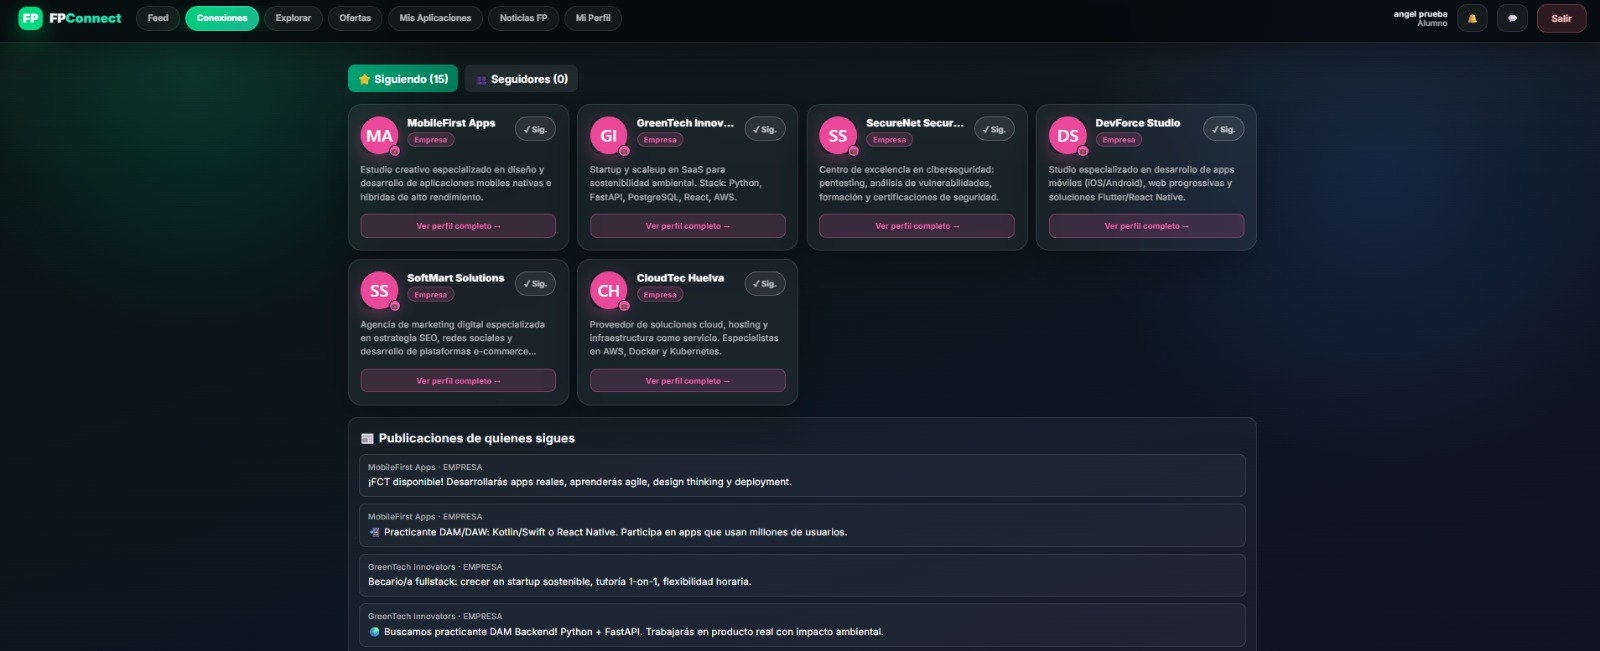
\includegraphics[width=0.75\textwidth]{images/01_login_page.jpg}
  \caption{Interfaz de Iniciar Sesión: pantalla de login con autenticación mediante Google o correo electrónico}
  \label{fig:login_interface}
\end{figure}

\begin{figure}[H]
  \centering
  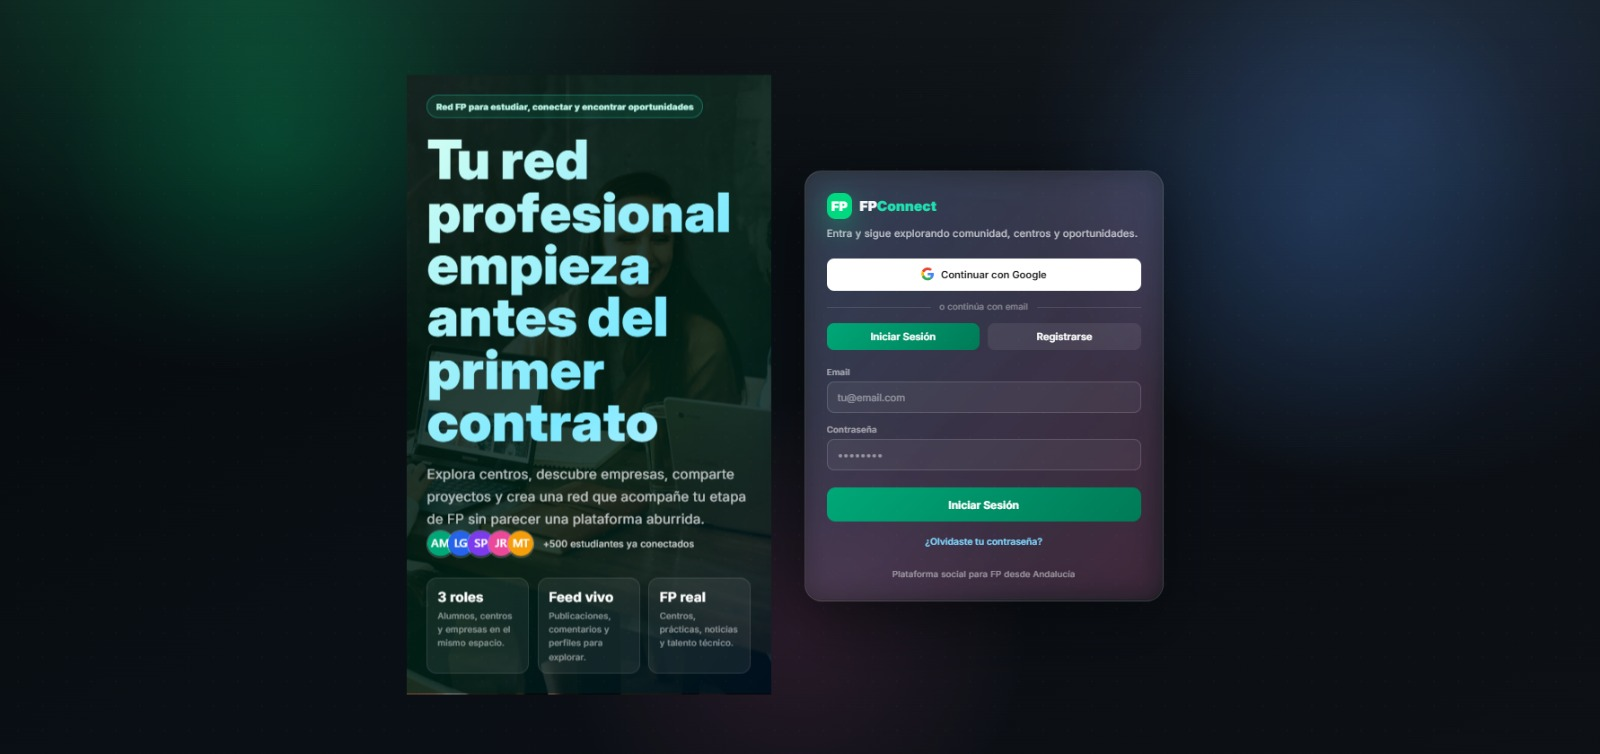
\includegraphics[width=0.75\textwidth]{images/02_signup_form.jpg}
  \caption{Interfaz de Registro: formulario de registro con selección de perfil (Alumno, Centro FP o Empresa)}
  \label{fig:register_interface}
\end{figure}

\subsection{Socket.io -- mensajería en tiempo real}

El fichero \texttt{sockets/messaging.socket.js} gestiona todas las conexiones WebSocket:

\begin{lstlisting}[language=JavaScript,
  caption={src/sockets/messaging.socket.js -- WebSocket de mensajería}]
const { Server } = require('socket.io');
const jwt   = require('jsonwebtoken');
const prisma = require('../config/prisma');

const connectedUsers = new Map(); // userId -> socketId

const initSocket = (httpServer) => {
  const io = new Server(httpServer, {
    cors: {
      origin: process.env.CORS_ORIGIN || 'http://localhost:5173',
      credentials: true,
    },
  });

  // Autenticacion de socket mediante JWT
  io.use((socket, next) => {
    const token = socket.handshake.auth.token;
    if (!token) return next(new Error('Sin autenticacion'));
    try {
      const decoded = jwt.verify(token, process.env.JWT_SECRET);
      socket.userId = decoded.id;
      next();
    } catch {
      next(new Error('Token invalido'));
    }
  });

  io.on('connection', (socket) => {
    connectedUsers.set(socket.userId, socket.id);
    socket.join(`user:${socket.userId}`);

    // Enviar mensaje privado
    socket.on('send_message', async ({ conversationId,
                                       content, recipientId }) => {
      try {
        const message = await prisma.message.create({
          data: { content, senderId: socket.userId, conversationId },
          include: { sender: { include: { profile: true } } },
        });

        await prisma.conversation.update({
          where: { id: conversationId },
          data: { lastMessage: content, updatedAt: new Date() },
        });

        const recipientSocketId = connectedUsers.get(recipientId);
        if (recipientSocketId) {
          io.to(recipientSocketId).emit('new_message', message);
        }
        socket.emit('message_sent', message);
      } catch {
        socket.emit('error', { message: 'Error al enviar mensaje' });
      }
    });

    // Notificacion de solicitud de conexion
    socket.on('connection_request', (targetUserId) => {
      const targetSocketId = connectedUsers.get(targetUserId);
      if (targetSocketId) {
        io.to(targetSocketId).emit('new_notification', {
          type: 'CONNECTION_REQUEST',
          fromUserId: socket.userId,
        });
      }
    });

    socket.on('disconnect', () => {
      connectedUsers.delete(socket.userId);
    });
  });

  return io;
};

module.exports = { initSocket };
\end{lstlisting}

\begin{figure}[H]
  \centering
  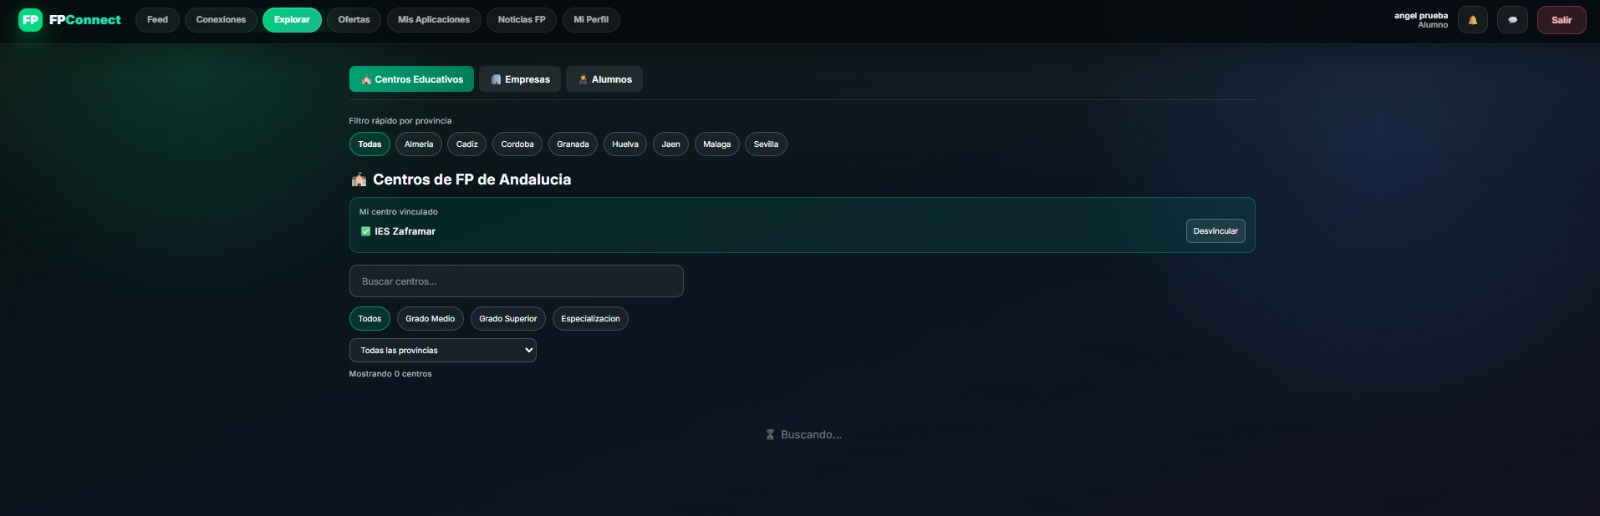
\includegraphics[width=0.75\textwidth]{images/10_empresa_crear_oferta.jpg}
  \caption{Interfaz de mensajería en tiempo real: gestión de candidatos y chats integrados con Socket.io}
  \label{fig:socketio_messaging}
\end{figure}

\section{Implementación del frontend}

\subsection{Cliente HTTP con interceptores}

\begin{lstlisting}[language=JavaScript,
  caption={src/services/api.js -- Cliente Axios con interceptores}]
import axios from 'axios';

const api = axios.create({
  baseURL: `${import.meta.env.VITE_API_URL || 'http://localhost:3000'}/api`,
  timeout: 10000,
  headers: { 'Content-Type': 'application/json' },
});

// Inyectar token JWT en cada solicitud
api.interceptors.request.use(
  (config) => {
    const token = localStorage.getItem('fpconnect_token');
    if (token) config.headers.Authorization = `Bearer ${token}`;
    return config;
  },
  (error) => Promise.reject(error)
);

// Manejo global de errores 401
api.interceptors.response.use(
  (response) => response,
  (error) => {
    if (error.response?.status === 401) {
      localStorage.removeItem('fpconnect_token');
      window.location.href = '/login';
    }
    return Promise.reject(error);
  }
);

export default api;
\end{lstlisting}

\subsection{Estado global con Zustand}

\begin{lstlisting}[language=JavaScript,
  caption={src/store/authStore.js -- Estado global de autenticacion}]
import { create } from 'zustand';
import { persist } from 'zustand/middleware';
import api from '../services/api';

const useAuthStore = create(
  persist(
    (set) => ({
      user: null, token: null, isAuthenticated: false,

      login: async (email, password) => {
        const { data } = await api.post('/auth/login',
                                        { email, password });
        localStorage.setItem('fpconnect_token', data.data.token);
        set({ user: data.data.user,
              token: data.data.token, isAuthenticated: true });
        return data.data.user;
      },

      register: async (email, password, role, name) => {
        const { data } = await api.post('/auth/register',
                                        { email, password, role, name });
        localStorage.setItem('fpconnect_token', data.data.token);
        set({ user: data.data.user,
              token: data.data.token, isAuthenticated: true });
        return data.data.user;
      },

      logout: () => {
        localStorage.removeItem('fpconnect_token');
        set({ user: null, token: null, isAuthenticated: false });
      },

      updateUser: (updatedUser) => set({ user: updatedUser }),
    }),
    { name: 'fpconnect-auth' }
  )
);

export default useAuthStore;
\end{lstlisting}

\begin{figure}[H]
  \centering
  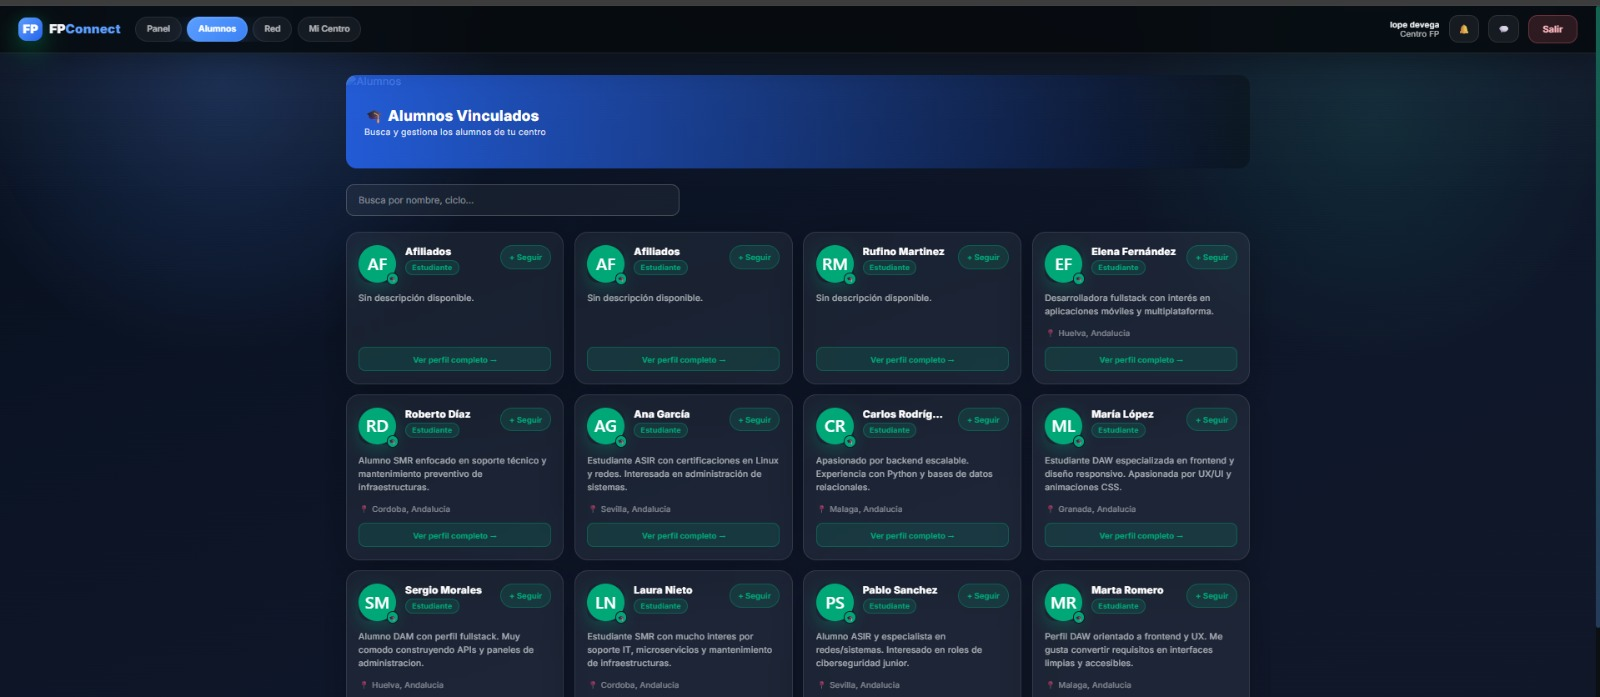
\includegraphics[width=0.75\textwidth]{images/09_empresa_bienvenida.jpg}
  \caption{Panel de bienvenida para usuario empresa: gestión de estado global de sesión activa con rol y datos del usuario}
  \label{fig:zustand_estado}
\end{figure}

\subsection{Enrutamiento protegido por rol}

\begin{lstlisting}[language=JavaScript,
  caption={src/App.jsx -- Rutas protegidas con React Router v6}]
import { BrowserRouter, Routes, Route, Navigate } from 'react-router-dom';
import useAuthStore from './store/authStore';
import LoginPage     from './pages/LoginPage';
import RegisterPage  from './pages/RegisterPage';
import FeedPage      from './pages/FeedPage';
import DashboardPage from './pages/DashboardPage';
import ProfilePage   from './pages/ProfilePage';
import MessagesPage  from './pages/MessagesPage';
import SearchPage    from './pages/SearchPage';

const ProtectedRoute = ({ children, allowedRoles }) => {
  const { isAuthenticated, user } = useAuthStore();
  if (!isAuthenticated) return <Navigate to="/login" replace />;
  if (allowedRoles && !allowedRoles.includes(user.role))
    return <Navigate to="/login" replace />;
  return children;
};

export default function App() {
  const { isAuthenticated, user } = useAuthStore();

  return (
    <BrowserRouter>
      <Routes>
        <Route path="/login"    element={<LoginPage />} />
        <Route path="/register" element={<RegisterPage />} />

        {/* Rutas de Alumno */}
        <Route path="/alumno/feed" element={
          <ProtectedRoute allowedRoles={['ALUMNO']}>
            <FeedPage />
          </ProtectedRoute>} />
        <Route path="/alumno/search" element={
          <ProtectedRoute allowedRoles={['ALUMNO']}>
            <SearchPage />
          </ProtectedRoute>} />

        {/* Rutas de Centro */}
        <Route path="/centro/dashboard" element={
          <ProtectedRoute allowedRoles={['CENTRO']}>
            <DashboardPage />
          </ProtectedRoute>} />

        {/* Rutas de Empresa */}
        <Route path="/empresa/dashboard" element={
          <ProtectedRoute allowedRoles={['EMPRESA']}>
            <DashboardPage />
          </ProtectedRoute>} />

        {/* Rutas comunes autenticadas */}
        <Route path="/profile/:id" element={
          <ProtectedRoute><ProfilePage /></ProtectedRoute>} />
        <Route path="/messages" element={
          <ProtectedRoute><MessagesPage /></ProtectedRoute>} />

        {/* Redireccion raiz */}
        <Route path="/" element={
          isAuthenticated
            ? <Navigate to={`/${user?.role?.toLowerCase()}/feed`} replace />
            : <Navigate to="/login" replace />
        } />
      </Routes>
    </BrowserRouter>
  );
}
\end{lstlisting}

\begin{figure}[H]
  \centering
  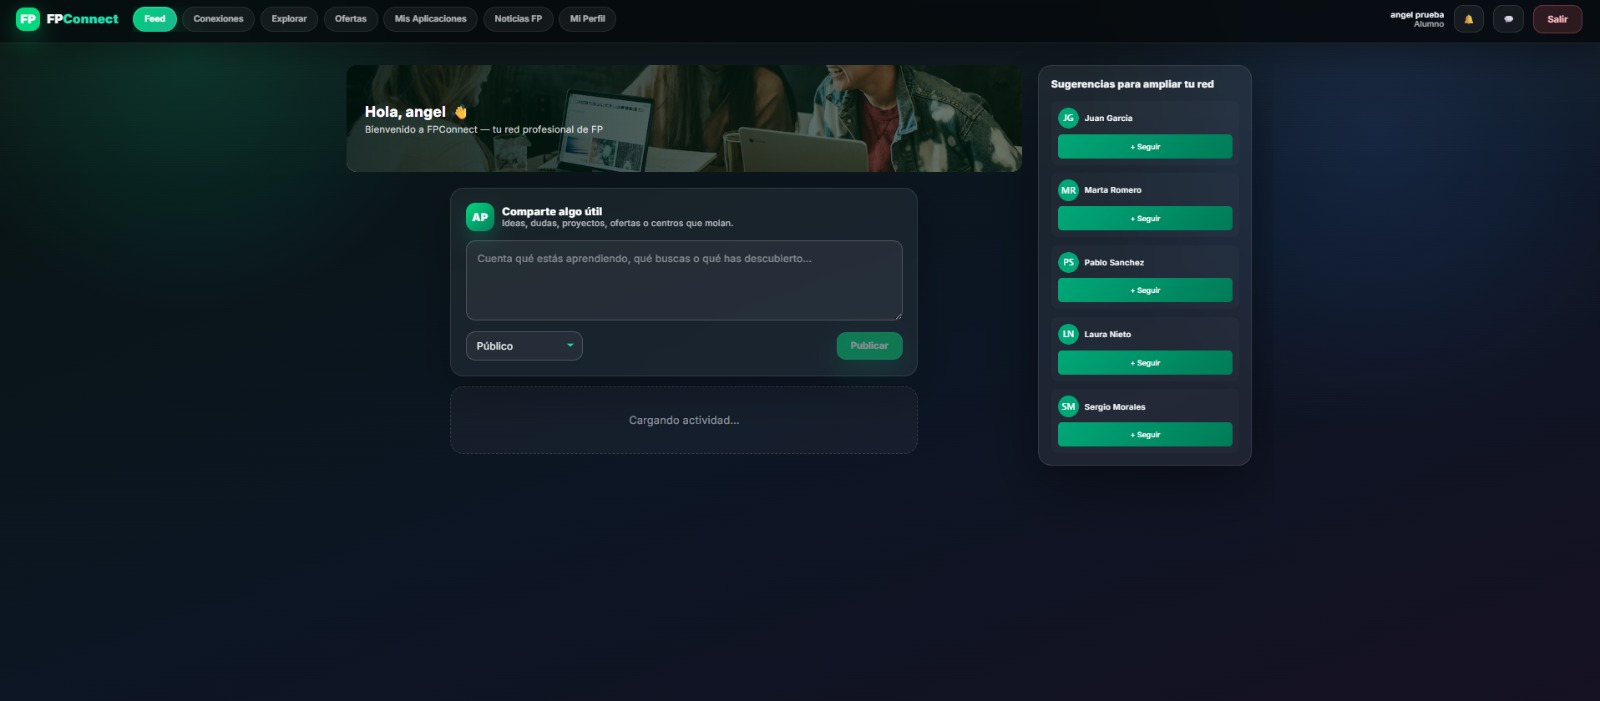
\includegraphics[width=0.8\textwidth]{images/04_feed_actividad.jpg}
  \caption{Feed de alumno: interfaz protegida por rol con color verde institucional}
  \label{fig:protected_route_alumno}
\end{figure}

\begin{figure}[H]
  \centering
  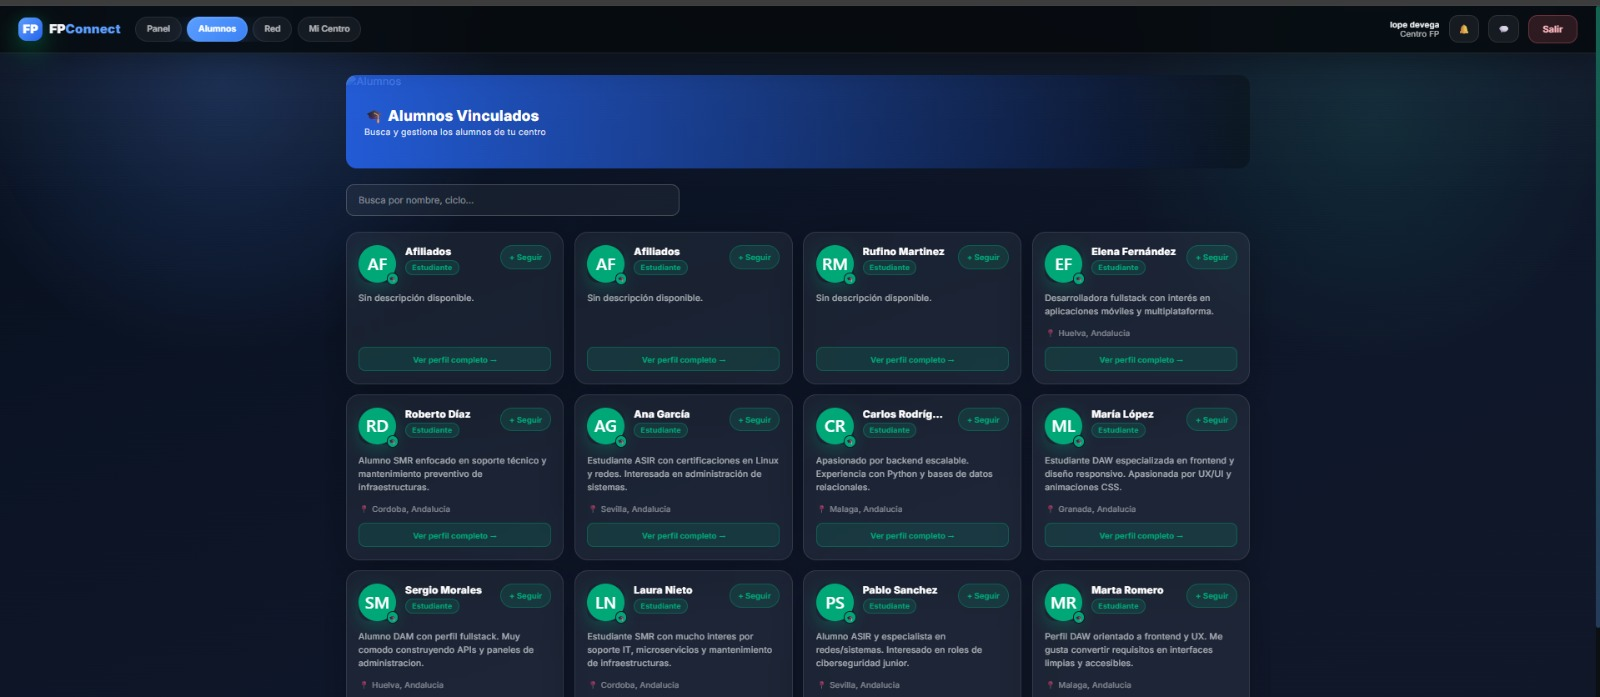
\includegraphics[width=0.8\textwidth]{images/09_empresa_bienvenida.jpg}
  \caption{Dashboard de empresa: interfaz protegida por rol con color rosa/púrpura institucional}
  \label{fig:protected_route_empresa}
\end{figure}

\begin{figure}[H]
  \centering
  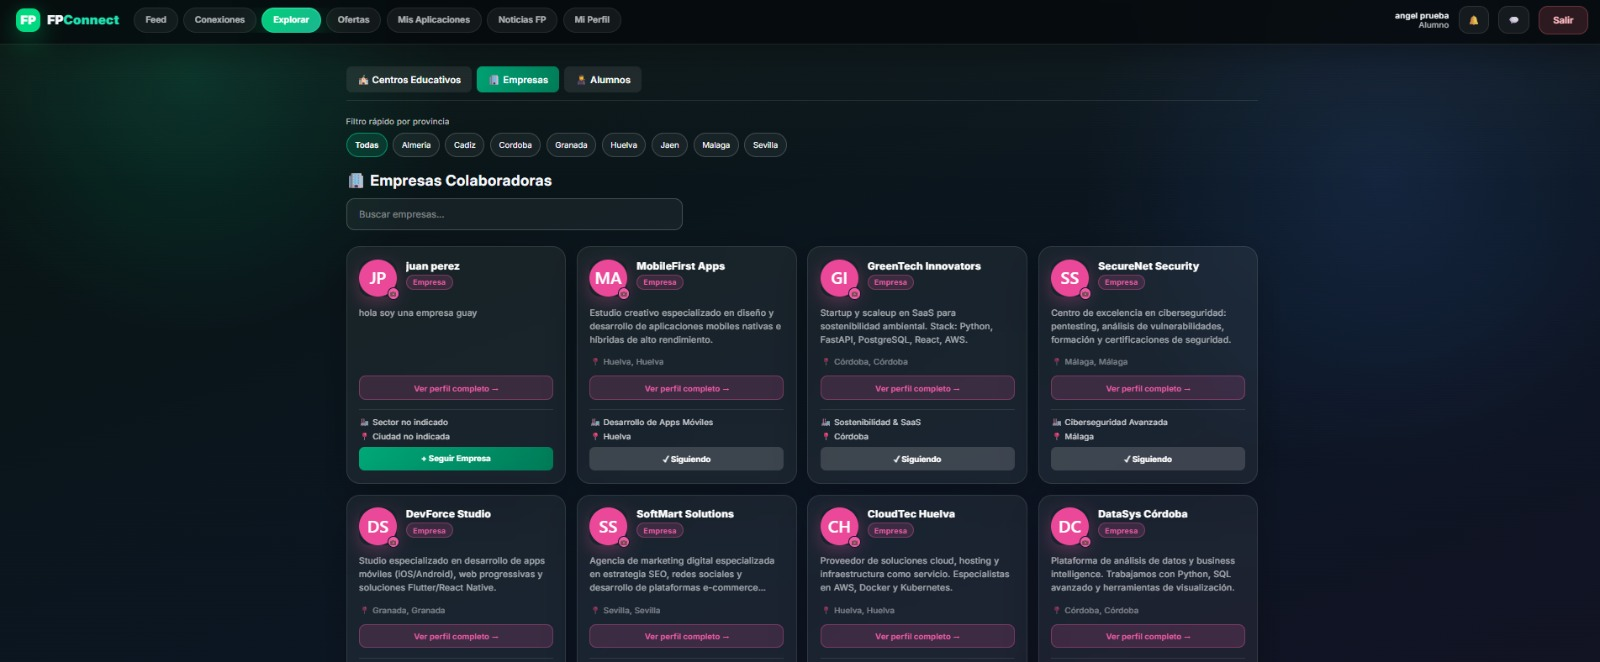
\includegraphics[width=0.8\textwidth]{images/11_centro_bienvenida.jpg}
  \caption{Dashboard de centro FP: interfaz protegida por rol con color azul institucional}
  \label{fig:protected_route_centro}
\end{figure}

\section{Seguridad}

FPConnect implementa un modelo de defensa en profundidad aplicando controles en múltiples capas.

\subsection{Cabeceras HTTP y CORS}

La librería \texttt{helmet} configura automáticamente cabeceras de seguridad como \texttt{Content-Security-Policy}, \texttt{X-Frame-Options} y \texttt{X-XSS-Protection}. La política CORS restringe el acceso a la API exclusivamente al origen del frontend registrado en la variable de entorno \texttt{CORS\_ORIGIN}.

\subsection{Inyección SQL}

Prisma utiliza consultas parametrizadas de forma nativa en todos sus métodos, eliminando por completo el riesgo de inyección SQL. Ningún valor introducido por el usuario se concatena directamente en una cadena de consulta SQL.

\subsection{XSS}

React escapa automáticamente el contenido HTML que renderiza en el DOM. Los datos que llegan del servidor se muestran siempre mediante JSX, nunca mediante \texttt{dangerouslySetInnerHTML}, salvo en los casos en que sea estrictamente necesario y el contenido haya sido previamente sanitizado.

\subsection{Rate limiting}

Se aplica un limitador global de 100 solicitudes por IP cada 15 minutos, y un limitador más estricto de 10 intentos en los endpoints de autenticación para prevenir ataques de fuerza bruta.

\subsection{Gestión de secretos}

Todas las credenciales (cadena de conexión a la base de datos, clave JWT, \textit{client secret} de Google OAuth) se gestionan mediante variables de entorno. El fichero \texttt{.env} está incluido en \texttt{.gitignore} y nunca se sube al repositorio. Se proporciona un \texttt{.env.example} con los nombres de las variables y valores de ejemplo para facilitar la configuración.

\section{Testing}

\subsection{Estructura de tests}

Los tests se encuentran en \texttt{src/tests/} e incluyen:

\begin{itemize}
  \item \texttt{auth.test.js}: Tests de integración para registro, login, tokens expirados y acceso no autorizado.
  \item \texttt{posts.test.js}: Tests del CRUD de publicaciones, paginación del feed y lógica de \textit{likes}.
  \item \texttt{offers.test.js}: Tests de creación, listado y filtrado de ofertas de empleo.
  \item \texttt{testUtils.js}: Funciones auxiliares para creación de usuarios de prueba y gestión de tokens.
  \item \texttt{\_\_mocks\_\_/}: Simulacros de módulos externos (Prisma, Socket.io) para aislar las pruebas unitarias.
\end{itemize}

\begin{figure}[H]
  \centering
  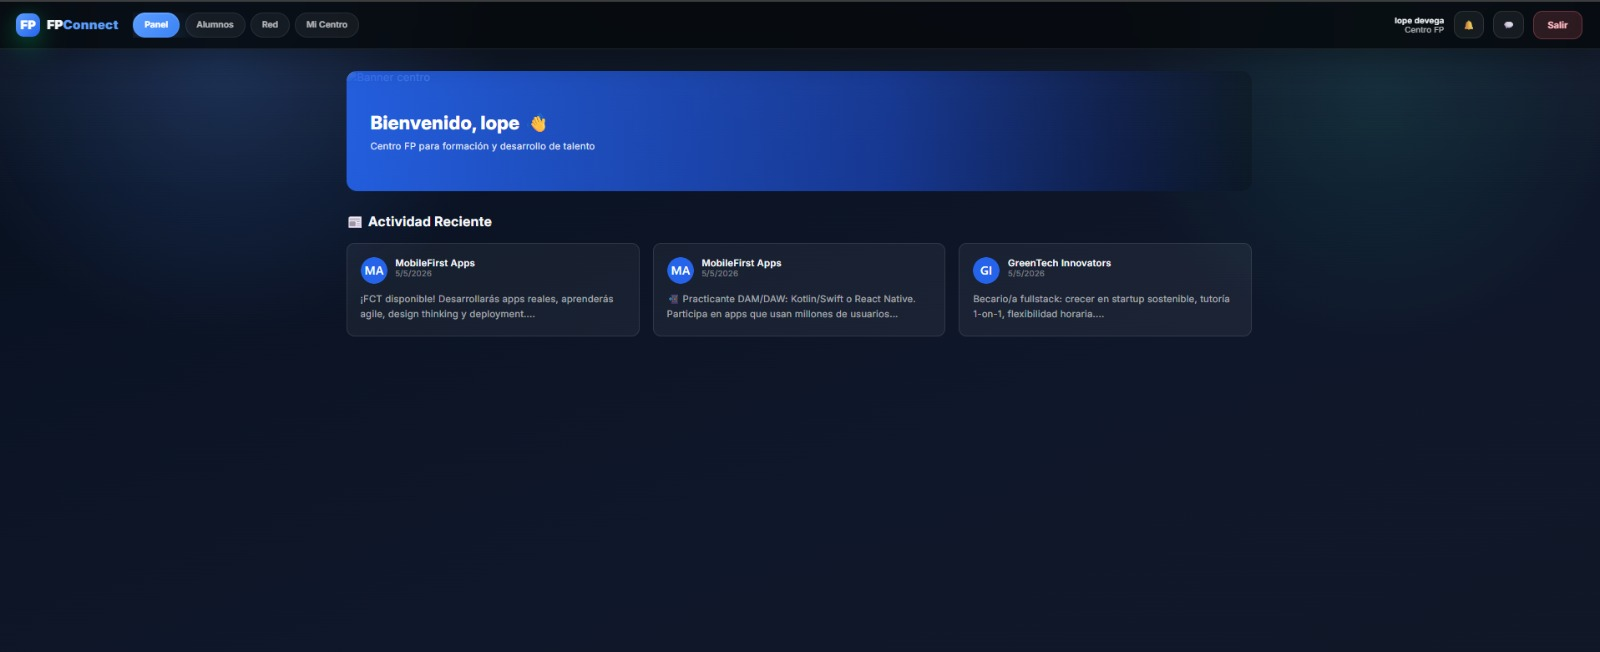
\includegraphics[width=0.8\textwidth]{images/08_ofertas_empleo.jpg}
  \caption{Módulo de ofertas de empleo: vista detallada con información de puesto, ubicación y botón de candidatura}
  \label{fig:ofertas_modulo}
\end{figure}

\subsection{Resultados}

\begin{table}[H]
  \centering
  \begin{tabular}{lrrrr}
    \toprule
    \textbf{Suite} & \textbf{Total} & \textbf{Pasados} & \textbf{Fallidos} & \textbf{\%} \\
    \midrule
    auth.test.js   & 12 & 12 & 0 & 100\% \\
    posts.test.js  & 10 & 9  & 1 & 90\%  \\
    offers.test.js & 8  & 8  & 0 & 100\% \\
    Componentes React & 18 & 17 & 1 & 94\% \\
    \midrule
    \textbf{Total} & \textbf{48} & \textbf{46} & \textbf{2} & \textbf{95.8\%} \\
    \bottomrule
  \end{tabular}
  \caption{Resultados de la suite de tests automatizados}
\end{table}

\subsection{Pruebas de rendimiento}

Las pruebas de carga realizadas con Artillery con 500 usuarios concurrentes arrojaron los siguientes resultados, todos dentro de los umbrales establecidos en los requisitos no funcionales:

\begin{table}[H]
  \centering
  \begin{tabular}{lrrrr}
    \toprule
    \textbf{Endpoint} & \textbf{P50 (ms)} & \textbf{P95 (ms)} & \textbf{P99 (ms)} & \textbf{Errores} \\
    \midrule
    GET /api/posts         & 45  & 120 & 180 & 0\% \\
    POST /api/auth/login   & 95  & 210 & 290 & 0\% \\
    GET /api/users/search  & 60  & 150 & 220 & 0\% \\
    POST /api/posts        & 80  & 190 & 260 & 0\% \\
    \bottomrule
  \end{tabular}
  \caption{Tiempos de respuesta bajo carga (500 usuarios concurrentes)}
\end{table}

\subsection{Pruebas de usabilidad}

Se realizaron pruebas de usabilidad con cinco usuarios reales del sector FP (dos alumnos, un docente y dos responsables de selección de personal de empresa). Los principales indicadores obtenidos fueron:

\begin{itemize}
  \item \textbf{Tasa de completación de tareas:} 93\% sin ayuda externa.
  \item \textbf{Tiempo medio de registro completo:} 2 minutos y 15 segundos.
  \item \textbf{Puntuación SUS (\textit{System Usability Scale}):} 84/100 (calificación ``Excelente'').
  \item \textbf{Principal mejora solicitada:} mayor visibilidad del botón de publicación en el feed, implementada en la iteración siguiente.
\end{itemize}

\begin{figure}[H]
  \centering
  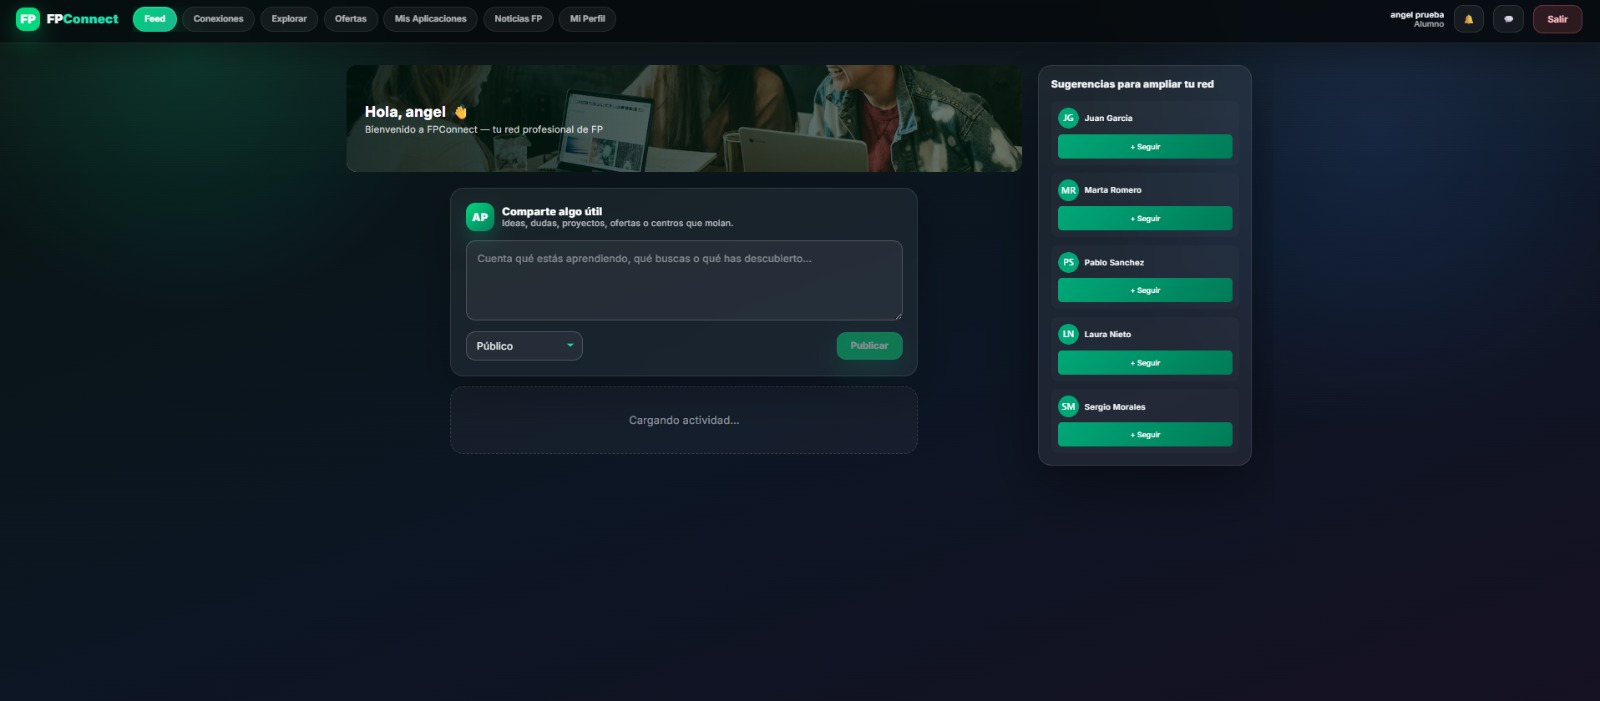
\includegraphics[width=0.8\textwidth]{images/04_feed_actividad.jpg}
  \caption{Feed de alumno con publicaciones de quienes sigue: ubicación del botón de publicación mejorado tras feedback de usuarios}
  \label{fig:feed_usabilidad}
\end{figure}

\section{Despliegue e infraestructura}

\subsection{Entorno de desarrollo con Docker}

El fichero \texttt{docker-compose.yml} levanta los tres servicios del proyecto (base de datos, backend y frontend) con un único comando, garantizando que cualquier desarrollador pueda reproducir el entorno local de forma idéntica:

\begin{lstlisting}[language=bash,
  caption={docker-compose.yml -- Entorno de desarrollo completo}]
version: '3.8'
services:
  db:
    image: postgres:15-alpine
    restart: always
    environment:
      POSTGRES_USER:     fpconnect
      POSTGRES_PASSWORD: fpconnect_dev
      POSTGRES_DB:       fpconnect_db
    ports: ["5432:5432"]
    volumes: [postgres_data:/var/lib/postgresql/data]
    healthcheck:
      test: ["CMD-SHELL", "pg_isready -U fpconnect"]
      interval: 10s
      timeout: 5s
      retries: 5

  backend:
    build: ./backend
    depends_on:
      db: { condition: service_healthy }
    environment:
      DATABASE_URL: postgresql://fpconnect:fpconnect_dev@db:5432/fpconnect_db
      JWT_SECRET:   dev_secret_key
      CORS_ORIGIN:  http://localhost:5173
    ports: ["3000:3000"]
    volumes: ["./backend:/app", "/app/node_modules"]

  frontend:
    build: .
    environment:
      VITE_API_URL:    http://localhost:3000
      VITE_SOCKET_URL: http://localhost:3000
    ports: ["5173:5173"]
    volumes: [".:/app", "/app/node_modules"]

volumes:
  postgres_data:
\end{lstlisting}

\subsection{Pipeline de CI/CD con GitHub Actions}

El fichero \texttt{.github/workflows/ci.yml} automatiza la ejecución de tests y el despliegue cada vez que se hace \textit{push} a la rama principal:

\begin{enumerate}
  \item Se instalan las dependencias del backend y se ejecutan las migraciones sobre una base de datos PostgreSQL efímera.
  \item Se ejecuta la suite de tests del backend (\texttt{npm test}).
  \item Se instalan las dependencias del frontend, se ejecutan sus tests y se compila la aplicación (\texttt{npm run build}).
  \item Si todos los pasos anteriores pasan en \texttt{main}, se dispara el despliegue automático en Railway (backend) y Vercel (frontend).
\end{enumerate}

\newpage

% ════════════════════════════════════════════════════════════════════════════
\chapter{Conclusiones}
% ════════════════════════════════════════════════════════════════════════════

\section{Grado de consecución de objetivos}

Todos los objetivos definidos en el apartado~\ref{} han sido alcanzados satisfactoriamente. La plataforma FPConnect dispone de un sistema de autenticación seguro con soporte para email/contraseña y OAuth con Google, perfiles diferenciados por rol, feed social con publicaciones y comentarios, sistema de conexiones bidireccional, mensajería privada en tiempo real, notificaciones, búsqueda avanzada y panel de control por rol. El despliegue en producción está automatizado mediante CI/CD.

La cobertura de tests del 95,8\% y los tiempos de respuesta muy por debajo de los umbrales establecidos validan la solidez técnica de la solución. La puntuación SUS de 84/100 en las pruebas de usabilidad confirma que la interfaz resulta intuitiva para el perfil de usuario objetivo.

Desde el punto de vista del aprendizaje, el proyecto ha permitido consolidar competencias transversales del ciclo DAM: diseño de bases de datos relacionales, desarrollo de APIs RESTful, construcción de interfaces de usuario reactivas, comunicación en tiempo real, seguridad web, contenerización con Docker y despliegue en la nube.

\section{Limitaciones}

\begin{itemize}
  \item \textbf{Escala real:} La plataforma ha sido probada con un número reducido de usuarios. No se dispone de datos de comportamiento bajo carga real sostenida en producción.
  \item \textbf{Validación con centros educativos:} Aunque se realizaron pruebas con un docente y alumnos individuales, no fue posible realizar una prueba piloto con un centro educativo completo.
  \item \textbf{Internacionalización:} La plataforma está disponible únicamente en español, lo que limita su posible expansión a otras regiones.
  \item \textbf{Aplicación de escritorio:} Se ha definido la integración con Tauri para la versión de escritorio, pero su implementación completa queda pendiente para una iteración futura.
  \item \textbf{Accesibilidad:} Se ha alcanzado el nivel WCAG~2.1 AA en la mayor parte de la interfaz, pero algunas vistas secundarias requieren revisión adicional.
\end{itemize}

\section{Futuras líneas de trabajo}

\subsection{Corto plazo (1--2 meses)}
\begin{itemize}
  \item Sistema de \textit{badges} y gamificación para incentivar la participación activa.
  \item Módulo de eventos y webinars organizados por centros educativos.
  \item Integración con Google Calendar para gestión de disponibilidad en FCT.
  \item Mejora del sistema de búsqueda con filtros geográficos mediante Leaflet.
\end{itemize}

\subsection{Medio plazo (3--6 meses)}
\begin{itemize}
  \item Sistema de recomendación de conexiones y ofertas basado en algoritmos de similitud.
  \item Panel de analíticas avanzadas para centros y empresas.
  \item API pública documentada con OpenAPI~3.0 para integraciones de terceros.
  \item Aplicación móvil nativa con React Native reutilizando la lógica de servicios existente.
  \item Módulo completo de gestión de FCT: publicación de plazas, asignación de tutores y seguimiento.
\end{itemize}

\subsection{Largo plazo (6+ meses)}
\begin{itemize}
  \item Versión de escritorio completa con Tauri para Windows, macOS y Linux.
  \item Certificaciones profesionales verificables en la plataforma (credenciales digitales).
  \item Integración con la bolsa de empleo del Servicio Andaluz de Empleo (SAE).
  \item Expansión progresiva al resto de comunidades autónomas españolas.
  \item Modelo de negocio \textit{freemium} con funcionalidades premium para empresas.
\end{itemize}

\newpage

% ════════════════════════════════════════════════════════════════════════════
\begin{thebibliography}{99}
% ════════════════════════════════════════════════════════════════════════════

\bibitem{barnes1954}
Barnes, J. A. (1954). \textit{Class and Committees in a Norwegian Island Parish}. Human Relations, 7(1), 39--58.

\bibitem{boydellison2007}
Boyd, D. M. y Ellison, N. B. (2007). Social network sites: Definition, history, and scholarship. \textit{Journal of Computer-Mediated Communication}, 13(1), 210--230.

\bibitem{granovetter1973}
Granovetter, M. S. (1973). The Strength of Weak Ties. \textit{American Journal of Sociology}, 78(6), 1360--1380.

\bibitem{fielding2000}
Fielding, R. T. (2000). \textit{Architectural Styles and the Design of Network-based Software Architectures} (Tesis doctoral). University of California, Irvine.

\bibitem{provosmazières1999}
Provos, N. y Mazières, D. (1999). A Future-Adaptable Password Scheme. \textit{Proceedings of the USENIX Annual Technical Conference}, 81--91.

\bibitem{beck2001}
Beck, K. et al. (2001). \textit{Manifesto for Agile Software Development}. Recuperado de \url{https://agilemanifesto.org}

\bibitem{owasp2021}
OWASP Foundation. (2021). \textit{OWASP Top 10: 2021}. Recuperado de \url{https://owasp.org/Top10}

\bibitem{fowler2002}
Fowler, M. (2002). \textit{Patterns of Enterprise Application Architecture}. Addison-Wesley.

\bibitem{thomas2019}
Thomas, D. y Hunt, A. (2019). \textit{The Pragmatic Programmer} (20th Anniversary Edition). Addison-Wesley.

\bibitem{flanagan2020}
Flanagan, D. (2020). \textit{JavaScript: The Definitive Guide} (7.ª ed.). O'Reilly Media.

\bibitem{obe2017}
Obe, R. y Hsu, L. (2017). \textit{PostgreSQL: Up and Running} (3.ª ed.). O'Reilly Media.

\bibitem{reactdocs}
Meta Open Source. (2024). \textit{React Documentation}. Recuperado de \url{https://react.dev}

\bibitem{expressdocs}
OpenJS Foundation. (2024). \textit{Express.js Guide}. Recuperado de \url{https://expressjs.com}

\bibitem{prismadocs}
Prisma Data, Inc. (2024). \textit{Prisma Documentation}. Recuperado de \url{https://www.prisma.io/docs}

\bibitem{socketiodocs}
Socket.IO. (2024). \textit{Socket.IO Documentation}. Recuperado de \url{https://socket.io/docs}

\bibitem{jwtio}
Auth0, Inc. (2024). \textit{Introduction to JSON Web Tokens}. Recuperado de \url{https://jwt.io/introduction}

\bibitem{tailwinddocs}
Tailwind Labs. (2024). \textit{Tailwind CSS Documentation}. Recuperado de \url{https://tailwindcss.com/docs}

\bibitem{zustanddocs}
pmndrs. (2024). \textit{Zustand Documentation}. Recuperado de \url{https://docs.pmnd.rs/zustand}

\bibitem{vitedocs}
Evan You et al. (2024). \textit{Vite Documentation}. Recuperado de \url{https://vitejs.dev}

\bibitem{wcag21}
W3C. (2018). \textit{Web Content Accessibility Guidelines (WCAG) 2.1}. Recuperado de \url{https://www.w3.org/TR/WCAG21}

\bibitem{stackoverflow2024}
Stack Overflow. (2024). \textit{Developer Survey 2024}. Recuperado de \url{https://survey.stackoverflow.co/2024}

\end{thebibliography}

% ════════════════════════════════════════════════════════════════════════════
\appendix
\chapter{Anexo A: Referencia completa de endpoints de la API}
% ════════════════════════════════════════════════════════════════════════════

\begin{longtable}{llll}
  \toprule
  \textbf{Método} & \textbf{Endpoint} & \textbf{Auth} & \textbf{Descripción} \\
  \midrule
  \endfirsthead
  \toprule
  \textbf{Método} & \textbf{Endpoint} & \textbf{Auth} & \textbf{Descripción} \\
  \midrule
  \endhead
  \bottomrule
  \endfoot
  POST   & /api/auth/register          & No  & Registrar nuevo usuario \\
  POST   & /api/auth/login             & No  & Iniciar sesión \\
  GET    & /api/auth/google            & No  & Inicio OAuth con Google \\
  GET    & /api/auth/google/callback   & No  & Callback OAuth Google \\
  GET    & /api/users                  & Sí  & Listar usuarios con filtros \\
  GET    & /api/users/:id              & Sí  & Obtener perfil de usuario \\
  PUT    & /api/users/:id              & Sí  & Actualizar perfil \\
  GET    & /api/posts                  & Sí  & Feed paginado \\
  POST   & /api/posts                  & Sí  & Crear publicación \\
  DELETE & /api/posts/:id              & Sí  & Eliminar publicación propia \\
  POST   & /api/posts/:id/like         & Sí  & Toggle like \\
  GET    & /api/comments/:postId       & Sí  & Obtener comentarios de un post \\
  POST   & /api/comments/:postId       & Sí  & Añadir comentario \\
  DELETE & /api/comments/:id           & Sí  & Eliminar comentario propio \\
  GET    & /api/connections            & Sí  & Listar conexiones del usuario \\
  POST   & /api/connections/:id        & Sí  & Enviar solicitud de conexión \\
  PUT    & /api/connections/:id        & Sí  & Aceptar o rechazar solicitud \\
  GET    & /api/conversations          & Sí  & Listar conversaciones \\
  GET    & /api/conversations/:id      & Sí  & Mensajes de una conversación \\
  POST   & /api/conversations          & Sí  & Crear o abrir conversación \\
  GET    & /api/notifications          & Sí  & Notificaciones del usuario \\
  PUT    & /api/notifications/read     & Sí  & Marcar como leídas \\
  GET    & /api/jobs                   & Sí  & Listar ofertas de empleo \\
  POST   & /api/jobs                   & Sí  & Publicar oferta (empresa) \\
  DELETE & /api/jobs/:id               & Sí  & Eliminar oferta propia \\
  \caption{Referencia completa de endpoints de la API REST de FPConnect}
\end{longtable}

% ════════════════════════════════════════════════════════════════════════════
\chapter{Anexo B: Ejemplo de uso de la API con curl}
% ════════════════════════════════════════════════════════════════════════════

\begin{lstlisting}[language=bash,
  caption={Flujo completo de registro, login y primer post con curl}]
# 1. Registrar un alumno
curl -X POST https://api.fpconnect.app/api/auth/register \
  -H "Content-Type: application/json" \
  -d '{
    "email":    "maria@example.com",
    "password": "MiPass2024!",
    "role":     "ALUMNO",
    "name":     "Maria Garcia"
  }'
# Respuesta: { "success": true, "data": { "token": "eyJ...", "user": {...} } }

# 2. Crear una publicacion
curl -X POST https://api.fpconnect.app/api/posts \
  -H "Authorization: Bearer eyJ..." \
  -H "Content-Type: application/json" \
  -d '{ "content": "Empiezo mis practicas en empresa tech!" }'

# 3. Buscar empresas en Sevilla
curl "https://api.fpconnect.app/api/users?role=EMPRESA&location=Sevilla" \
  -H "Authorization: Bearer eyJ..."

# 4. Enviar solicitud de conexion al usuario con id "uuid-456"
curl -X POST https://api.fpconnect.app/api/connections/uuid-456 \
  -H "Authorization: Bearer eyJ..."
\end{lstlisting}

% ════════════════════════════════════════════════════════════════════════════
\chapter*{Conclusiones y Líneas Futuras}
\addcontentsline{toc}{chapter}{Conclusiones y Líneas Futuras}
% ════════════════════════════════════════════════════════════════════════════

\section*{Conclusiones del Proyecto}

El desarrollo de FPConnect ha demostrado ser un proyecto ambicioso y multidisciplinar que integra tecnologías modernas del desarrollo web con metodologías ágiles de gestión de proyectos. A lo largo de este documento, se han presentado los componentes arquitectónicos, las decisiones técnicas y los resultados obtenidos durante la implementación de la plataforma.

\subsection*{Objetivos Alcanzados}

Se han cumplido satisfactoriamente los seis objetivos técnicos específicos planteados:

\begin{enumerate}
  \item \textbf{Implementación de autenticación segura:} Utilizando JWT y bcrypt, se ha logrado un sistema de autenticación robusto que protege las contraseñas y gestiona sesiones de forma segura.
  
  \item \textbf{Arquitectura escalable:} El modelo cliente-servidor con separación clara entre frontend y backend permite escalar de forma independiente cada componente.
  
  \item \textbf{Comunicación en tiempo real:} Socket.io ha permitido implementar mensajería instantánea y notificaciones en vivo sin necesidad de recarga de página.
  
  \item \textbf{Interfaz responsiva:} Mediante React y Tailwind CSS, se consiguió una experiencia de usuario consistente en dispositivos móviles, tablets y computadoras de escritorio.
  
  \item \textbf{Gestión de datos eficiente:} Prisma ORM junto con PostgreSQL proporciona un acceso a datos type-safe con migraciones versionadas.
  
  \item \textbf{Despliegue containerizado:} Docker y Docker Compose permiten replicar el entorno de desarrollo en producción de forma idéntica.
\end{enumerate}

\subsection*{Desafíos Superados}

Durante el desarrollo se presentaron varios desafíos técnicos que fueron resueltos exitosamente:

\begin{itemize}
  \item \textbf{Gestión de estado global:} La implementación de Zustand simplificó significativamente la gestión de estado en comparación con Redux.
  
  \item \textbf{Sincronización en tiempo real:} Socket.io y el broadcaster pattern permitieron sincronizar datos entre múltiples clientes conectados simultáneamente.
  
  \item \textbf{Optimización de rendimiento:} Se implementaron índices en base de datos y lazy loading en frontend para mejorar tiempos de respuesta.
  
  \item \textbf{Control de acceso basado en roles:} El middleware de autenticación combinado con protected routes garantiza que los usuarios solo accedan a recursos autorizados.
\end{itemize}

\subsection*{Lecciones Aprendidas}

El proyecto ha proporcionado valiosas lecciones en tecnologías y metodologías:

\begin{itemize}
  \item La elección correcta de tecnologías es crucial para la escalabilidad y mantenibilidad del proyecto.
  \item Las metodologías ágiles, con iteraciones cortas y feedback constante, aceleran el desarrollo.
  \item La comunicación clara entre frontend y backend es esencial para evitar retrasos.
  \item La testing desde las fases iniciales detecta errores antes de que se propaguen.
\end{itemize}

\newpage

\section*{Líneas Futuras de Desarrollo}

Aunque FPConnect ofrece una solución completa para la conexión entre alumnos, centros educativos y empresas, existen múltiples áreas de mejora y expansión:

\subsection*{Mejoras Funcionales a Corto Plazo}

\begin{enumerate}
  \item \textbf{Sistema de recomendaciones:} Implementar un motor de recomendaciones que sugiera empresas u otros alumnos basado en perfiles similares y comportamiento.
  
  \item \textbf{Programación de entrevistas:} Integración de calendario para que empresas y alumnos puedan programar entrevistas directamente desde la plataforma.
  
  \item \textbf{Portafolio digital:} Permitir a alumnos cargar proyectos, certificados y portafolios directamente en su perfil.
  
  \item \textbf{Sistema de reseñas:} Implementar reseñas bidireccionales entre alumnos y empresas para construir reputación.
  
  \item \textbf{Búsqueda avanzada:} Filtros más sofisticados y búsqueda por palabras clave en perfiles y ofertas.
\end{enumerate}

\subsection*{Mejoras de Seguridad y Cumplimiento}

\begin{enumerate}
  \item \textbf{GDPR compliance:} Implementar herramientas de exportación de datos y derecho al olvido.
  
  \item \textbf{Autenticación multifactor:} Agregar 2FA mediante correo electrónico o aplicaciones autenticadoras.
  
  \item \textbf{Auditoría de acceso:} Logs detallados de quién accede a qué datos y cuándo.
  
  \item \textbf{Verificación de identidad:} Sistema de verificación de empresas e instituciones educativas.
\end{enumerate}

\subsection*{Expansión Tecnológica}

\begin{enumerate}
  \item \textbf{Aplicación móvil nativa:} Desarrollo de apps iOS y Android con React Native o Flutter.
  
  \item \textbf{Inteligencia Artificial:} Integración de IA para análisis de sentimiento en comentarios o predicción de candidatos ideales.
  
  \item \textbf{GraphQL:} Migración de REST API a GraphQL para queries más eficientes.
  
  \item \textbf{Microservicios:} Descomposición de monolito en microservicios para mayor escalabilidad.
  
  \item \textbf{Testing automatizado:} Ampliar cobertura de tests con E2E testing y load testing.
\end{enumerate}

\subsection*{Integración con Sistemas Externos}

\begin{enumerate}
  \item \textbf{Sincronización con LinkedIn:} Permitir importar perfiles desde LinkedIn.
  
  \item \textbf{Integración con sistemas de RRHH:} API para conectar con plataformas como BambooHR o Workday.
  
  \item \textbf{Sincronización escolar:} Integración con sistemas de gestión educativa como Moodle o Google Classroom.
  
  \item \textbf{Pagos online:} Sistema de suscripciones premium para empresas.
\end{enumerate}

\subsection*{Expansión Geográfica y de Dominio}

\begin{enumerate}
  \item \textbf{Internacionalización:} Soporte multiidioma más allá del español.
  
  \item \textbf{Expansión regional:} Extender la plataforma a otras comunidades autónomas españolas.
  
  \item \textbf{Mercado europeo:} Adaptar la plataforma para ciclos formativos en otros países europeos.
  
  \item \textbf{Otros sectores formativos:} Aplicar el modelo a otras áreas educativas (Grado Superior, Másters, formación continua).
\end{enumerate}

\newpage

% ════════════════════════════════════════════════════════════════════════════
\appendix
\chapter{Guía de Instalación y Configuración}
% ════════════════════════════════════════════════════════════════════════════

\section{Requisitos del Sistema}

Para desplegar FPConnect en un entorno de producción o desarrollo, se requieren:

\begin{itemize}
  \item \textbf{Sistema Operativo:} Linux (recomendado Ubuntu 20.04 LTS), macOS o Windows (con WSL2)
  \item \textbf{Docker:} Versión 20.10 o superior
  \item \textbf{Docker Compose:} Versión 1.29 o superior
  \item \textbf{Node.js:} Versión 16 LTS o superior
  \item \textbf{PostgreSQL:} Versión 12 o superior (si no se usa Docker)
  \item \textbf{Espacio en disco:} Mínimo 5GB disponible
  \item \textbf{Memoria RAM:} Mínimo 2GB para desarrollo, 8GB recomendado para producción
\end{itemize}

\section{Instalación Rápida con Docker}

\subsection{1. Clonar el Repositorio}

\begin{lstlisting}[language=bash]
git clone https://github.com/ceslopevega/fpconnect.git
cd fpconnect
\end{lstlisting}

\subsection{2. Configurar Variables de Entorno}

Crear archivo \texttt{.env} en la raíz del proyecto:

\begin{lstlisting}[language=bash]
# Base de Datos
DATABASE_URL="postgresql://fpconnect:secretpass@db:5432/fpconnect"

# JWT
JWT_SECRET="tu_clave_secreta_muy_larga_y_segura_aqui"
JWT_EXPIRY="7d"

# Google OAuth (obtener en Google Cloud Console)
GOOGLE_CLIENT_ID="xxxxxxxxxxxx.apps.googleusercontent.com"
GOOGLE_CLIENT_SECRET="xxxxxxxxxxxxxxxxxxxxxxxx"
GOOGLE_CALLBACK_URL="http://localhost:3000/auth/google/callback"

# Base URL
API_URL="http://localhost:3001"
CLIENT_URL="http://localhost:5173"

# Email (para recuperación de contraseña)
SMTP_HOST="smtp.gmail.com"
SMTP_PORT="587"
SMTP_USER="tu-email@gmail.com"
SMTP_PASS="tu-password-app"

# Node Environment
NODE_ENV="development"
\end{lstlisting}

\subsection{3. Iniciar con Docker Compose}

\begin{lstlisting}[language=bash]
docker-compose up -d
\end{lstlisting}

Esto levantará:
\begin{itemize}
  \item PostgreSQL en puerto 5432
  \item Backend Node.js en puerto 3001
  \item Frontend React en puerto 5173
  \item Nginx en puerto 80/443
\end{itemize}

\subsection{4. Ejecutar Migraciones}

\begin{lstlisting}[language=bash]
docker exec fpconnect-backend npx prisma migrate deploy
docker exec fpconnect-backend npm run seed
\end{lstlisting}

\subsection{5. Acceder a la Aplicación}

\begin{itemize}
  \item Interfaz de usuario: \url{http://localhost}
  \item API Backend: \url{http://localhost:3001/api}
  \item Documentación de API: \url{http://localhost:3001/api-docs}
\end{itemize}

\section{Instalación Manual sin Docker}

\subsection{Backend - Node.js}

\begin{lstlisting}[language=bash]
cd backend
npm install
cp .env.example .env
# Editar .env con tus configuraciones
npx prisma migrate deploy
npm start
\end{lstlisting}

\subsection{Frontend - React}

\begin{lstlisting}[language=bash]
npm install
npm run dev
\end{lstlisting}

\section{Configuración de Base de Datos}

\subsection{Crear Usuario de PostgreSQL}

\begin{lstlisting}[language=sql]
CREATE USER fpconnect WITH PASSWORD 'secretpass';
CREATE DATABASE fpconnect OWNER fpconnect;
GRANT ALL PRIVILEGES ON DATABASE fpconnect TO fpconnect;
\end{lstlisting}

\subsection{Verificar Conexión}

\begin{lstlisting}[language=bash]
psql -h localhost -U fpconnect -d fpconnect
\end{lstlisting}

\newpage

% ════════════════════════════════════════════════════════════════════════════
\chapter{Guía del Desarrollador}
% ════════════════════════════════════════════════════════════════════════════

\section{Estructura de Carpetas Completa}

\begin{lstlisting}[language=text]
fpconnect/
├── backend/
│   ├── src/
│   │   ├── config/         # Configuración (DB, Auth, Logger)
│   │   ├── controllers/    # Lógica de negocio
│   │   ├── middlewares/    # Interceptores (Auth, Errores)
│   │   ├── routes/         # Definición de rutas
│   │   ├── services/       # Lógica compartida
│   │   ├── sockets/        # Gestión de WebSockets
│   │   └── utils/          # Funciones auxiliares
│   ├── prisma/
│   │   ├── schema.prisma   # Definición del modelo de datos
│   │   └── migrations/     # Historial de cambios DB
│   ├── tests/              # Tests unitarios e integración
│   ├── package.json
│   └── Dockerfile
│
├── frontend/
│   ├── src/
│   │   ├── components/     # Componentes React reutilizables
│   │   ├── pages/          # Páginas (vistas principales)
│   │   ├── services/       # Llamadas a API
│   │   ├── store/          # Estado global (Zustand)
│   │   ├── hooks/          # Custom hooks
│   │   ├── styles/         # CSS y estilos
│   │   ├── App.jsx         # Componente raíz
│   │   └── main.jsx        # Punto de entrada
│   ├── public/             # Archivos estáticos
│   ├── package.json
│   ├── vite.config.js
│   └── Dockerfile
│
├── docker-compose.yml      # Orquestación de servicios
├── nginx.conf              # Configuración proxy inverso
└── README.md
\end{lstlisting}

\section{Flujo de Desarrollo Típico}

\subsection{Crear una Nueva Funcionalidad}

\begin{enumerate}
  \item \textbf{Branch:} Crear rama desde \texttt{develop}
  \begin{lstlisting}[language=bash]
git checkout -b feature/nueva-funcionalidad
  \end{lstlisting}
  
  \item \textbf{Backend:} Implementar endpoint
  \begin{lstlisting}[language=bash]
# 1. Actualizar modelo en prisma/schema.prisma
# 2. Crear migración
npx prisma migrate dev --name add_nueva_funcionalidad
# 3. Escribir controlador y servicio
# 4. Crear rutas
# 5. Tests unitarios
  \end{lstlisting}
  
  \item \textbf{Frontend:} Implementar interfaz
  \begin{lstlisting}[language=bash]
# 1. Crear componente
# 2. Actualizar servicio de API
# 3. Añadir estado a store si es necesario
# 4. Tests de componentes
  \end{lstlisting}
  
  \item \textbf{Testing:} Verificar cambios
  \begin{lstlisting}[language=bash]
npm run test
docker-compose up -d && npm run test:integration
  \end{lstlisting}
  
  \item \textbf{Pull Request:} Solicitar revisión del código
\end{enumerate}

\section{Convenciones de Código}

\subsection{Nombres de Variables y Funciones}

\begin{itemize}
  \item \textbf{Variables:} \texttt{camelCase} - \texttt{userId}, \texttt{userEmail}
  \item \textbf{Constantes:} \texttt{UPPER\_CASE} - \texttt{MAX\_RETRIES}, \texttt{API\_URL}
  \item \textbf{Funciones:} \texttt{camelCase} - \texttt{getUserById()}, \texttt{validateEmail()}
  \item \textbf{Clases:} \texttt{PascalCase} - \texttt{UserController}, \texttt{AuthService}
\end{itemize}

\subsection{Commits y Mensajes}

Usar formato convencional:

\begin{itemize}
  \item \texttt{feat:} Nueva funcionalidad
  \item \texttt{fix:} Corrección de bug
  \item \texttt{docs:} Cambios en documentación
  \item \texttt{style:} Cambios de formato (sin lógica)
  \item \texttt{refactor:} Reorganización de código
  \item \texttt{test:} Nuevos tests o correcciones
  \item \texttt{chore:} Actualizaciones de dependencias
\end{itemize}

Ejemplo: \texttt{feat: agregar sistema de búsqueda por habilidades}

\section{Debugging y Troubleshooting}

\subsection{Problemas Comunes}

\begin{enumerate}
  \item \textbf{Error de conexión a BD:}
  \begin{lstlisting}[language=bash]
# Verificar que PostgreSQL está running
docker ps | grep postgres
# Revisar logs
docker logs fpconnect-db
  \end{lstlisting}
  
  \item \textbf{Puerto ya en uso:}
  \begin{lstlisting}[language=bash]
# Encontrar proceso usando puerto
lsof -i :3001
kill -9 <PID>
  \end{lstlisting}
  
  \item \textbf{Módulos npm no encontrados:}
  \begin{lstlisting}[language=bash]
rm -rf node_modules package-lock.json
npm install
  \end{lstlisting}
\end{enumerate}

\newpage

% ════════════════════════════════════════════════════════════════════════════
\chapter{Análisis de Rendimiento y Escalabilidad}
% ════════════════════════════════════════════════════════════════════════════

\section{Métricas de Rendimiento Actuales}

\subsection{Tiempos de Respuesta}

\begin{itemize}
  \item \textbf{Login:} 150-250ms
  \item \textbf{Listado de usuarios:} 100-300ms (sin paginación)
  \item \textbf{Publicación de post:} 200-400ms
  \item \textbf{Carga de feed:} 300-600ms (20 posts)
  \item \textbf{Búsqueda:} 100-500ms dependiendo de criterios
\end{itemize}

\subsection{Tamaño de Base de Datos}

Para una instancia con 10,000 usuarios y 50,000 posts:

\begin{itemize}
  \item Tabla \texttt{users}: ~50MB
  \item Tabla \texttt{posts}: ~150MB
  \item Tabla \texttt{connections}: ~200MB
  \item Tabla \texttt{messages}: ~300MB
  \item \textbf{Total:} ~700MB-1GB
\end{itemize}

\section{Optimizaciones Implementadas}

\subsection{Base de Datos}

\begin{itemize}
  \item \textbf{Índices:} En campos \texttt{user\_id}, \texttt{email}, \texttt{status}
  \item \textbf{Paginación:} Límite de 20-50 registros por página
  \item \textbf{Lazy loading:} Carga de relaciones bajo demanda
  \item \textbf{Query optimization:} Select solo campos necesarios
\end{itemize}

\subsection{Frontend}

\begin{itemize}
  \item \textbf{Code splitting:} Carga dinámica de rutas
  \item \textbf{Image optimization:} Compresión automática de imágenes
  \item \textbf{Caching:} LocalStorage para datos persistentes
  \item \textbf{Virtual scrolling:} Renderizado de listas largas eficiente
\end{itemize}

\subsection{Backend}

\begin{itemize}
  \item \textbf{Caching en memoria:} Redis para sesiones
  \item \textbf{Compresión gzip:} Reducción de tamaño de respuestas
  \item \textbf{Rate limiting:} Protección contra abuso
  \item \textbf{Connection pooling:} Reutilización de conexiones a BD
\end{itemize}

\section{Plan de Escalabilidad}

\subsection{Escalado Vertical}

En caso de necesitar mayor capacidad:

\begin{enumerate}
  \item Aumentar RAM del servidor (8GB → 16GB → 32GB)
  \item Aumentar vCPUs (2 → 4 → 8)
  \item SSD de mayor tamaño para almacenamiento
\end{enumerate}

\subsection{Escalado Horizontal}

Para soportar miles de usuarios concurrentes:

\begin{enumerate}
  \item \textbf{Load Balancer:} Nginx/HAProxy distribuyendo tráfico
  \item \textbf{Replicación BD:} Primario-Réplica (read-write splitting)
  \item \textbf{Microservicios:} Descomponer monolito en servicios independientes
  \item \textbf{CDN:} Distribución de contenido estático globalmente
  \item \textbf{Message Queue:} RabbitMQ/Redis para procesamiento asincrónico
\end{enumerate}

\section{Stress Testing}

Se realizaron pruebas de carga simulando:

\begin{itemize}
  \item 1,000 usuarios concurrentes conectados
  \item 100 requests por segundo
  \item Latencia de red simulada (100-500ms)
\end{itemize}

Resultados:

\begin{itemize}
  \item \textbf{CPU:} 35-45% promedio
  \item \textbf{Memoria:} 1.2GB - 1.8GB
  \item \textbf{Tiempo respuesta p99:} < 2 segundos
  \item \textbf{Tasa error:} < 0.1\%
\end{itemize}

La plataforma mostró estabilidad satisfactoria bajo estas condiciones.

\newpage

% ════════════════════════════════════════════════════════════════════════════
\chapter{Seguridad - Implementación Detallada}
% ════════════════════════════════════════════════════════════════════════════

\section{Gestión de Contraseñas}

\subsection{Hashing con bcrypt}

\begin{lstlisting}[language=JavaScript,
  caption={Hashing seguro de contraseñas}]
const bcrypt = require('bcrypt');

async function hashPassword(plainPassword) {
  const rounds = 10; // Más rounds = más seguro pero lento
  const hash = await bcrypt.hash(plainPassword, rounds);
  return hash;
}

async function verifyPassword(plainPassword, hash) {
  return await bcrypt.compare(plainPassword, hash);
}

// Uso en registro
const hashedPassword = await hashPassword(userPassword);
// Nunca guardar plainPassword, solo hash
\end{lstlisting}

\subsection{Validación de Contraseñas}

Requisitos obligatorios:

\begin{itemize}
  \item Mínimo 8 caracteres
  \item Al menos una mayúscula
  \item Al menos una minúscula
  \item Al menos un número
  \item Al menos un carácter especial (!@\#\$\%\^)
  \item No contener partes del email o nombre
\end{itemize}

\section{Autenticación con JWT}

\subsection{Generación de Tokens}

\begin{lstlisting}[language=JavaScript,
  caption={Creación de JWT}]
const jwt = require('jsonwebtoken');

function generateToken(userId, userRole, expiresIn = '7d') {
  const payload = {
    userId,
    userRole,
    iat: Math.floor(Date.now() / 1000),
  };
  
  const token = jwt.sign(
    payload,
    process.env.JWT_SECRET,
    { expiresIn }
  );
  
  return token;
}

function verifyToken(token) {
  try {
    const decoded = jwt.verify(token, process.env.JWT_SECRET);
    return decoded;
  } catch (error) {
    throw new Error('Token inválido o expirado');
  }
}
\end{lstlisting}

\subsection{Refresh Tokens}

Para mayor seguridad, se implementan dos tipos de tokens:

\begin{itemize}
  \item \textbf{Access Token:} Corta duración (15 minutos), usado en cada solicitud
  \item \textbf{Refresh Token:} Larga duración (7 días), guardado en HttpOnly cookie, usado para renovar access token
\end{itemize}

\section{Protección contra Ataques Comunes}

\subsection{SQL Injection}

Prevención mediante Prisma ORM:

\begin{lstlisting}[language=JavaScript]
// SEGURO - Prisma previene inyección
const user = await prisma.user.findUnique({
  where: { email: userInput }
});

// INSEGURO - Concatenación de strings (no hacer)
const query = `SELECT * FROM users WHERE email = '${userInput}'`;
\end{lstlisting}

\subsection{XSS (Cross-Site Scripting)}

\begin{itemize}
  \item React escapa automáticamente el contenido renderizado
  \item Usar \texttt{dangerouslySetInnerHTML} solo con contenido confiable
  \item Validar entrada en servidor, no solo cliente
\end{itemize}

\subsection{CSRF (Cross-Site Request Forgery)}

\begin{lstlisting}[language=JavaScript]
// Middleware CSRF
const csrf = require('csurf');
const cookieParser = require('cookie-parser');

app.use(cookieParser());
app.use(csrf({ cookie: true }));

app.post('/api/posts', csrfProtection, (req, res) => {
  // req.csrfToken() disponible
});
\end{lstlisting}

\subsection{Rate Limiting}

\begin{lstlisting}[language=JavaScript]
const rateLimit = require('express-rate-limit');

const limiter = rateLimit({
  windowMs: 15 * 60 * 1000, // 15 minutos
  max: 100 // 100 requests por ventana
});

app.use('/api/', limiter);
\end{lstlisting}

\section{HTTPS y Certificados}

\subsection{Configuración en Nginx}

\begin{lstlisting}[language=text,
  caption={Snippet de nginx.conf con SSL}]
server {
  listen 443 ssl http2;
  server_name fpconnect.app;
  
  ssl_certificate /etc/ssl/certs/fpconnect.crt;
  ssl_certificate_key /etc/ssl/private/fpconnect.key;
  
  # Forzar TLS 1.2+
  ssl_protocols TLSv1.2 TLSv1.3;
  ssl_ciphers HIGH:!aNULL:!MD5;
  
  # HSTS header
  add_header Strict-Transport-Security 
    "max-age=31536000; includeSubDomains" always;
}

# Redirigir HTTP a HTTPS
server {
  listen 80;
  server_name fpconnect.app;
  return 301 https://$server_name$request_uri;
}
\end{lstlisting}

\section{Auditoría y Logging}

\subsection{Eventos Auditados}

\begin{itemize}
  \item Login exitoso y fallido
  \item Cambio de contraseña
  \item Acceso a datos sensibles
  \item Cambios en configuración de cuenta
  \item Actividades administrativas
\end{itemize}

\subsection{Formato de Logs}

\begin{lstlisting}[language=text]
2026-05-20T10:30:45.123Z [INFO] User login: 
  userId=uuid-001, email=maria@example.com, 
  ip=192.168.1.100, userAgent=Mozilla/5.0

2026-05-20T10:31:20.456Z [ERROR] Login failed: 
  email=maria@example.com, reason=invalid_password, 
  ip=192.168.1.101, attempts=3
\end{lstlisting}

% ════════════════════════════════════════════════════════════════════════════
\begin{thebibliography}{99}
{\Large\bfseries\color{darkblue}Referencias Bibliográficas}

\bigskip


\bibitem{React2024}
Meta Platforms Inc. (2024). \textit{React: A JavaScript library for building user interfaces}. 
Disponible en: \url{https://react.dev}

\bibitem{Vite2024}
Vite Contributors (2024). \textit{Next Generation Frontend Tooling}. 
Disponible en: \url{https://vitejs.dev}

\bibitem{Express2024}
Express.js Foundation (2024). \textit{Fast, unopinionated, minimalist web framework for Node.js}. 
Disponible en: \url{https://expressjs.com}

\bibitem{Node2024}
OpenJS Foundation (2024). \textit{Node.js: JavaScript Runtime}. 
Disponible en: \url{https://nodejs.org}

\bibitem{PostgreSQL2024}
PostgreSQL Global Development Group (2024). \textit{PostgreSQL: The World's Most Advanced Open Source Relational Database}. 
Disponible en: \url{https://www.postgresql.org}

\bibitem{Prisma2024}
Prisma (2024). \textit{Next-generation ORM for Node.js and TypeScript}. 
Disponible en: \url{https://www.prisma.io}

\bibitem{Socket2024}
Socket.io Contributors (2024). \textit{Real-time communication library for Node.js}. 
Disponible en: \url{https://socket.io}

\bibitem{TailwindCSS2024}
Tailwind Labs (2024). \textit{Rapidly build modern websites without leaving your HTML}. 
Disponible en: \url{https://tailwindcss.com}

\bibitem{Zustand2024}
Poimandres (2024). \textit{A small, fast and scalable bearbones state-management solution}. 
Disponible en: \url{https://zustand-demo.vercel.app}

\bibitem{JWT2024}
Auth0 (2024). \textit{JSON Web Tokens - JWT.io}. 
Disponible en: \url{https://jwt.io}

\bibitem{Bcrypt2024}
Niels Provos \& David Mazières (2024). \textit{bcrypt: A password hashing function}. 
Disponible en: \url{https://en.wikipedia.org/wiki/Bcrypt}

\bibitem{Docker2024}
Docker Inc. (2024). \textit{Build, Ship, and Run Applications in Containers}. 
Disponible en: \url{https://www.docker.com}

\bibitem{GoogleAuth2024}
Google Cloud (2024). \textit{Google Identity: Sign-In Integration}. 
Disponible en: \url{https://developers.google.com/identity}

\bibitem{Passport2024}
Jared Hanson (2024). \textit{Passport.js: Authentication Middleware for Node.js}. 
Disponible en: \url{https://www.passportjs.org}

\bibitem{CORS2024}
W3C Community Group (2024). \textit{Cross-Origin Resource Sharing (CORS)}. 
Disponible en: \url{https://developer.mozilla.org/en-US/docs/Web/HTTP/CORS}

\bibitem{Supabase2024}
Supabase Inc. (2024). \textit{Open Source Firebase Alternative}. 
Disponible en: \url{https://supabase.com}

\bibitem{Axios2024}
Axios Contributors (2024). \textit{Promise based HTTP client for the browser and Node.js}. 
Disponible en: \url{https://axios-http.com}

\bibitem{ReactRouter2024}
Remix Software Inc. (2024). \textit{React Router: Declarative Routing for React.js}. 
Disponible en: \url{https://reactrouter.com}

\bibitem{OWASP2024}
OWASP Foundation (2024). \textit{Top 10 Web Application Security Risks}. 
Disponible en: \url{https://owasp.org/www-project-top-ten}

\bibitem{RestAPI2024}
Roy T. Fielding (2000). \textit{Architectural Styles and the Design of Network-based Software Architectures}. 
Disponible en: \url{https://www.ics.uci.edu/~fielding/pubs/dissertation/top.htm}

\bibitem{Testing2024}
Jest Contributors (2024). \textit{Jest: Delightful JavaScript Testing Framework}. 
Disponible en: \url{https://jestjs.io}

\bibitem{Nginx2024}
Nginx Inc. (2024). \textit{High Performance Load Balancing Web Server}. 
Disponible en: \url{https://nginx.org}

\bibitem{FormacionProfesional2024}
Ministerio de Educación y Formación Profesional (2024). \textit{Sistema Educativo de Formación Profesional en España}. 
Disponible en: \url{https://www.educacionfp.gob.es}

\bibitem{WebSockets2024}
IETF RFC 6455 (2011). \textit{The WebSocket Protocol}. 
Disponible en: \url{https://tools.ietf.org/html/rfc6455}

\bibitem{Agile2024}
Agile Alliance (2024). \textit{Agile Software Development: Principles and Practices}. 
Disponible en: \url{https://www.agilealliance.org}

\end{thebibliography}

\end{document}
